\chapter{Applikations-Architektur}

\section{Software Architektur Grundbegriffe}

Nachfolgend die Definition von Software Architektur:

\begin{quote}
Die Architektur eines Softwaresystems besteht aus seinen Strukturen, der Zerlegung in Komponenten, deren Schnittstellen und Beziehungen untereinander.
\end{quote}

Die Definition baut wiederum auf dem Systembegriff auf, welcher eine Gesamtheit von Elementen mit klarer Abgrenzung zu seiner Umwelt ist. Daraus folgt, dass eine Architektur die Komponenten eines Systems definieren muss. Zudem sollten die Beziehungen zwischen diesen Komponenten charakterisiert und die wesentlichen Merkmale des Systems beschrieben werden. Dabei wird zwischen den statischen (Bauplan) und dynamischen Aspekten (Ablaufplan) unterschieden.

Es werden verschiedene Arten von Architekten unterschieden. Der Infrastructre Architect modelliert das \textit{Versorgungsnetz} des Systems. Der Enterprise Architect hat den Überblick über das grosse Ganze und entwirft sozusagen den \textit{Stadtplan}. In dieser Zusammenfassung konzentrieren wir uns aber auf den Application Architect (auch Solution Architect), der den \textit{Hausplan} entwirft.

Wie in der Bauarchitektur wird der Stil einer Softwarearchitektur von den Anforderung getrieben. Möchte man ein Gebäude zur Verteidigung erstellen, baut man keinen ästhetischen Glasturm, sondern ein solides Bollwerk aus Stein. Auch auf dem Bau existieren meist mehrere Lösungen für das ein und dasselbe Problem. Möchte man z.B. eine mobile Unterkunft kann man ein Zelt mitnehmen oder in einem Wohnwagen schlafen. Beides hat seine Vor- bzw. Nachteile. Es gibt aber auch Unterschiede zwischen Bau- und Softwarearchitektur. So lässt sich Software z.B. fast beliebig oft Umbauen ohne grösseren Schaden anzurichten. Das fördert eine iterative, inkrementelle Vorgehensweise. Das grosse Problem der Softwarearchitektur ist, dass man nicht einfach davor stehen kann um sie zu sehen wie bei der Gebäudearchitektur.

Das oberste Ziel einer guten Architektur ist eine Reduzierung der Komplexität. Diese Reduzierung kann z.B. durch Zerlegung in Komponenten, durch Abstraktion, Wiederverwendung oder einer guten Dokumentation erreicht werden. Die Bedeutung einer guten Architektur nimmt zu, weil heutige Systeme meist hochkomplex und integriert sind sowie sich laufend an neue Anforderungen anpassen müssen. Abbildung \ref{fig:begriffe} zeigt einen Überblick über die wichtigsten Begriffe für einen Architekten.

\begin{figure}
\centering
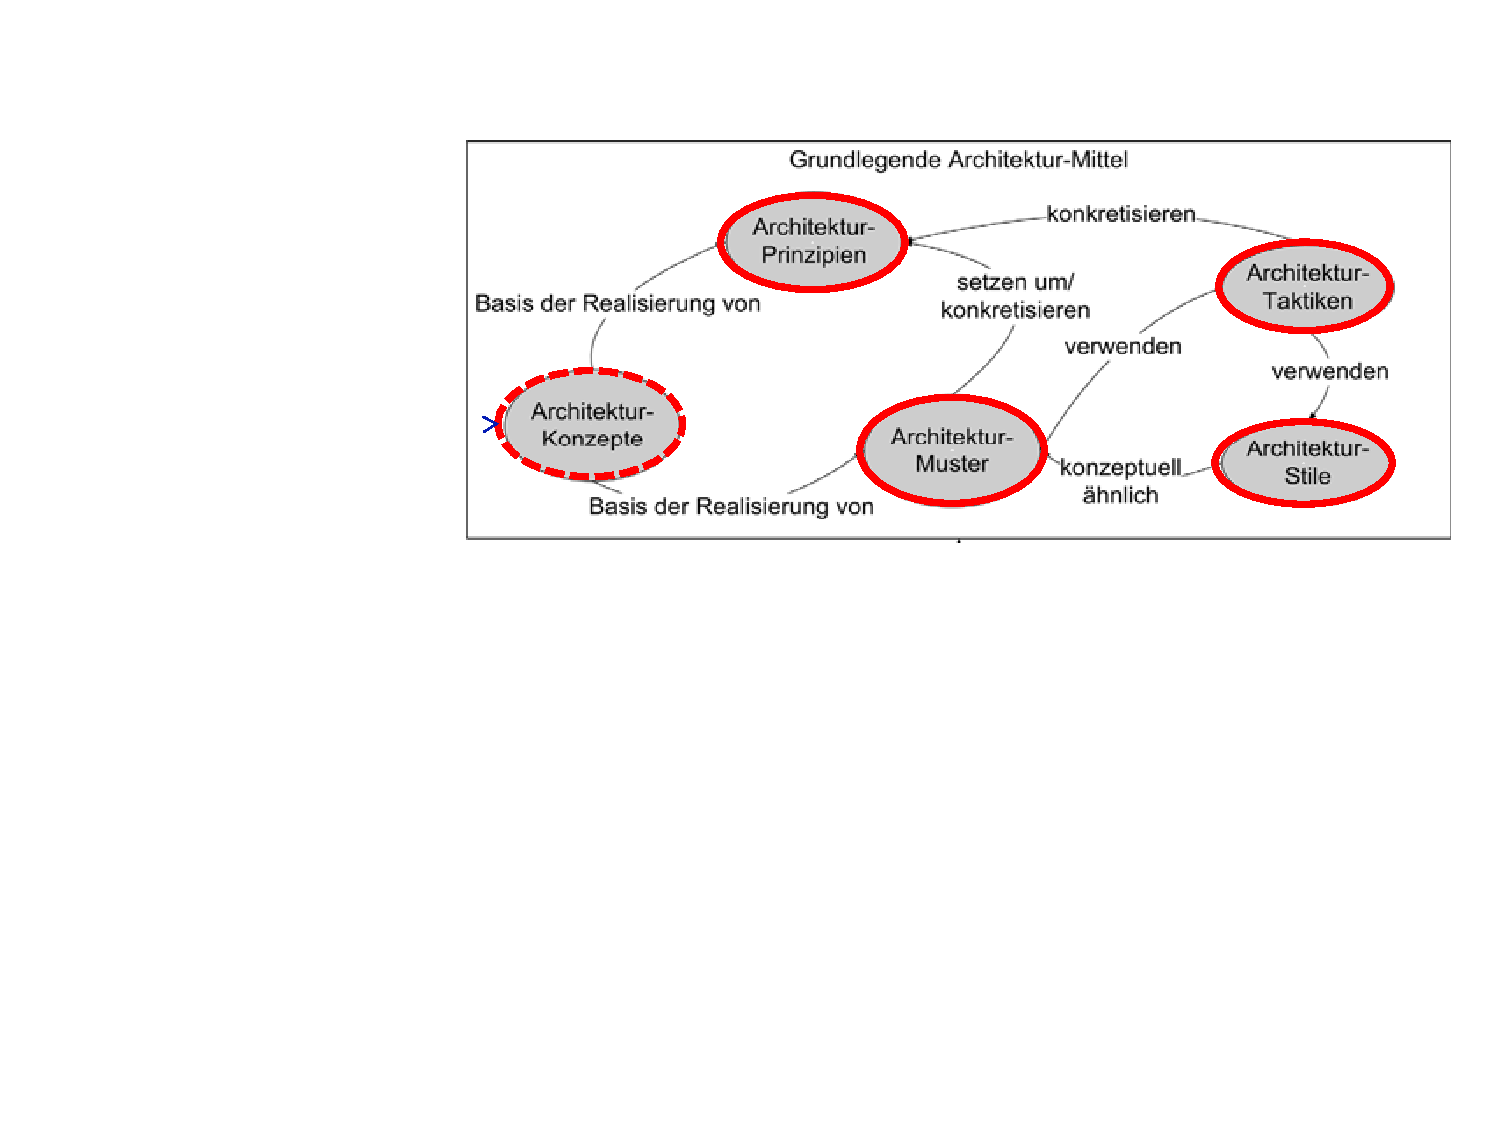
\includegraphics[width=0.6\linewidth]{fig/begriffe}
\caption{Grundlegende Begriffe}
\label{fig:begriffe}
\end{figure}

Bei einem Architekturentwurf werden Anforderungen, Qualitätsmerkmale und Rahmenbedingungen in den Prozess hineingegeben und heraus kommt eine Architektur welche durchführbar und entwicklungsfähig ist. Um so eine Architektur hinzukriegen, werden die Methoden in Abbildung \ref{fig:begriffe} angewendet. Abbildung \ref{fig:twin-peaks} zeigt das erweitere Twin Peaks Modell. Es soll aufzeigen dass die Architektur der \textbf{Vermittler} zwischen Anforderungen und Konstruktion ist. Zudem wird das ganze System in einem iterativen Prozess entworfen, was die Spirale darstellen soll.

\begin{figure}
\centering
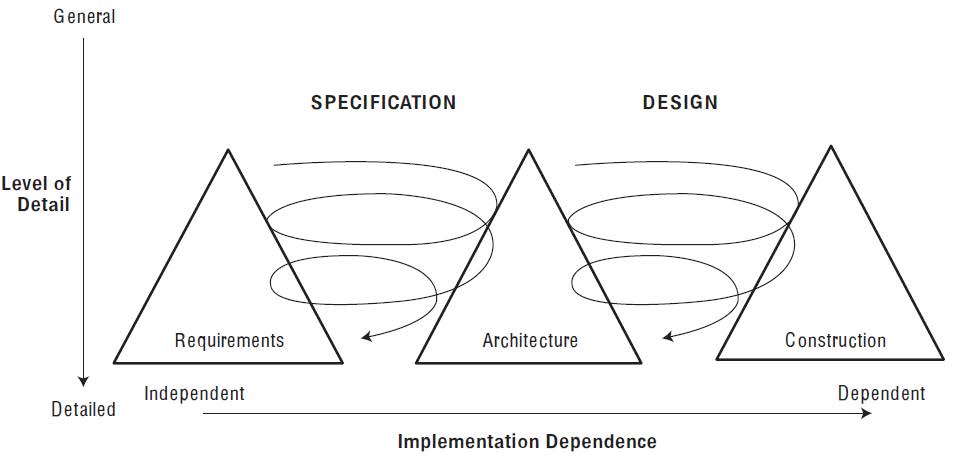
\includegraphics[width=0.7\linewidth]{fig/twin-peaks}
\caption{Erweitertes Twin Peaks Modell}
\label{fig:twin-peaks}
\end{figure}

Der iterative, inkrementelle Prozess des Architekturentwurfs läuft immer gleich ab:
\begin{enumerate}
	\item Analyse der Anforderungen und Auflösung von Konflikten
	\item Anwendung von Prinzipien, Taktiken \& Mustern
	\item Treffen von Entscheidungen \& Kompromissen
	\item Bewertung von Alternativen
	\item Bereitstellen von Sichten für Beteiligte
	\item Dokumentation und Bewertung von Entscheidungen
	\item Wenn Entwurf ok umsetzen sonst \verb|goto 1|
\end{enumerate}
Zum Schluss: Jedes System hat eine Architektur auch wenn keine Beschreibung ausserhalb des Codes existiert und sie in der Implementierung schwer zu erkennen ist.

Der Verfall von Software tritt ein, wenn das System zunehmend mit neuen Funktionen ausgestattet wird ohne sich dabei neue Gedanken über die Architektur zu machen. Das ist ein natürlicher Prozess, welche anschliessend ein Refactoring erfordert.

Der Unterschied zwischen Architektur und Design lässt sich gut an einem Beispiel ausmachen: Der Architekt definiert, dass die Komponente eine REST-Schnittstelle anbietet. Der Software-Entwickler setzt diese Schnittstelle konkret um - welche Ressourcen, welche Parameter usw.

\section{Requirement-Engineering}
Jedes Software-Projekt steht und fällt mit den Anforderungen. Karl Wiegers und Joy Beatty sagen, dass die Anforderungen nicht gleich ins kleinste Detail bekannt sein müssen, sondern nur immer soweit, dass das Entwicklungs-Team mit dem nächsten Schritt fortfahren kann. Zudem muss man sich immer bewusst sein, dass das was der Kunde sagt, oft nicht das ist was er meint.

In den letzten Jahren hat die Business-Analyse an Bedeutung gewonnen. Doch unterschätzt man allgemein immer noch die Wichtigkeit des Requirement-Engineering. Die Architektur sieht man als Brücke zwischen den Geschäftszielen und dem Software-System.

Inhärente (angeboren, innewohnend) Schwierigkeiten bei der Anforderungsanalyse:
\begin{itemize}
	\item Verständnis: Stakeholder können nicht wirklich wissen was sie wollen (im Sinne der IT Lösung).
	\item Kommunikation: Komplex, unklar, Business-IT Gap
	\item Kontrolle: Schwierig für den Software-Entwicklungsprozess
	\item Nichttrennbare Verantwortlichkeiten: Alles scheint von allem abzuhängen
\end{itemize}

Zufällige Schwierigkeiten bei der Anforderungsanalyse:
\begin{itemize}
	\item Anforderungen später schreiben: nicht hilfreich für die Entwicklung (aber: rapid prototyping)
	\item Widersprüchliche Interessen: Marketing (hype), allg. Dokumentation (unabh. von Anforderungen), Verträge. Das ist die Aufgabe des Architekten!
	\item Ungenügende Anstrengungen, weil ich vielleicht keinen Bock haben mit Person X zu reden.
	\item Unentdeckt: Schlichtweg vergessen oder unbekannt.
\end{itemize}

Anforderungen müssen SMART sein. SMART bedeutet:
\begin{description}
	\item[Specific:] Eindeutig und konsistent (Beschrieben mit angemessenem Detaillierungsgrad)
	\item[Measurable:] Messbar (Wie kann beurteilt werden, ob die Anforderung erreicht wurde?)
	\item[Attainable:] Erreichbar (Technisch machbar mit dem aktuellen Stand der Technik)
	\item[Realizable:] Umsetzbar (Unter den gegebenen Randbedingungen und verfügbare Ressourcen)
	\item[Traceable:] Nachverfolgbar (Konzeption - Spezifikation - Design - Implementation - Test)
\end{description}

\begin{figure}[h!]
\centering
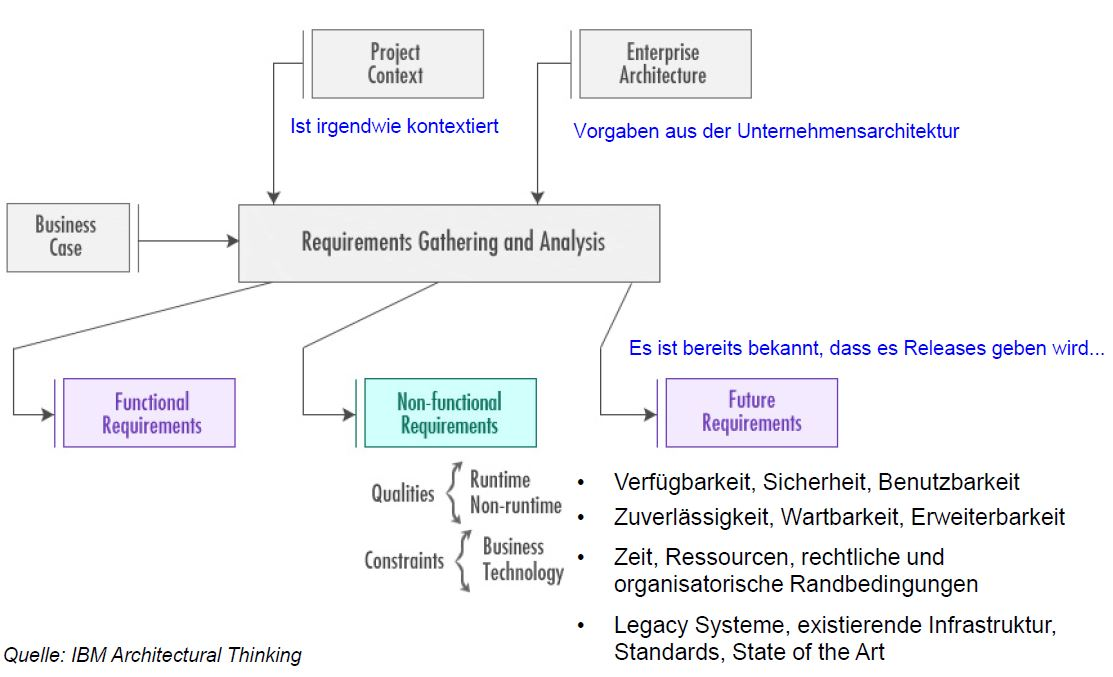
\includegraphics[width=0.75\linewidth]{fig/requirements-gathering-and-analysis}
\caption{Requriements Gathering and Analysis}
\label{fig:requirements-gathering-and-analysis}
\end{figure}

\section{Funktionale Anforderungen: Use cases und User Stories}
\label{sec:funktionale-anforderungen}

Bei funktionalen Anforderung steht die Systemfunktionalität im Zentrum. Was bietet es mir, was kann ich damit tun? 

Um funktionale Anforderungen aufzunehmen gibt es grundsätzlich zwei Mittel: User Story und Use Cases. Den Unterschied zwischen den beiden Arten beschreibe ich gerne wie folgt: Eine User Story ist ein leichtgewichtiges Planungsinstrument, welches den Dialog mit dem Kunden fördert. Ein Use Case ist ein schwergewichtiges Dokumentationsinstrument in welchem die Anforderung detailliert spezifiziert wird. Die User-Story sind mehr Business getrieben die Use Cases sind eher auf der technischen Seite anzusiedeln.

Falls eine User Story zu gross erscheint, kann diese als Epic angesehen werden. Wobei das Epic dann in mehrere User Storys unterteilt wird. Eine User Story hat das Muster \emph{“As a [role] I can [function] so that [rationale].”}. Gute User Stories sind INVEST (Independent, Negotiable, Valuable, Estimatable, Small, Testable). Zudem hat jeder User Story entsprechende Akzeptanzkriterien (Definition of Done).

Oft macht man folgende Fehler beim verfassen von User Stories: Too formal or too much detail, Technical tasks masquerading as stories, Skipping the conversation.

Nachfolgend ein Use-Case Template:

\begin{figure}[h!]
\centering
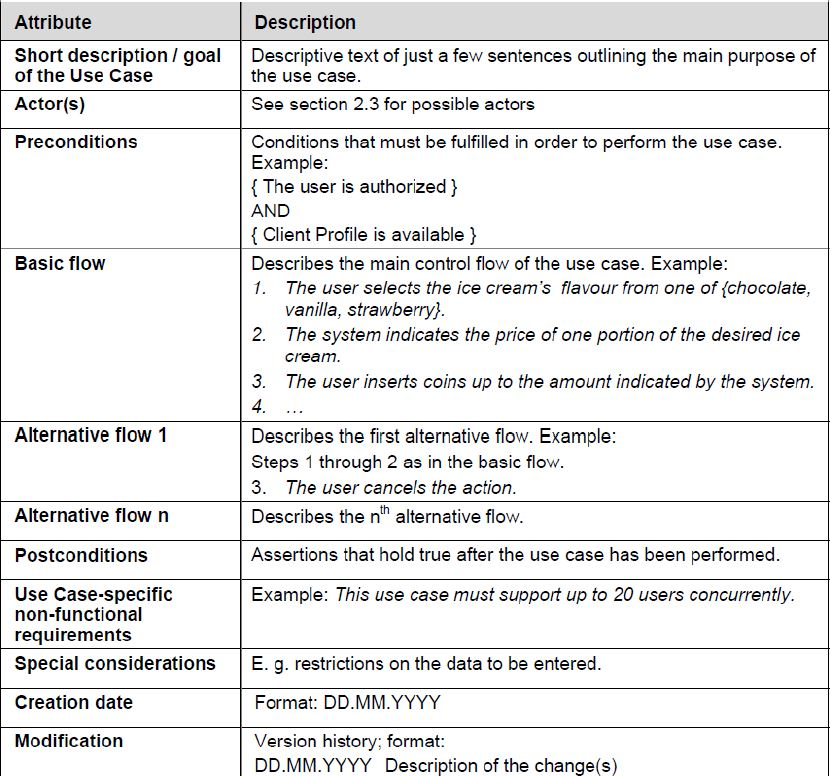
\includegraphics[width=0.7\linewidth]{fig/use-case-template}
\caption{Use Case Template}
\label{fig:use-case-template}
\end{figure}

\newpage
Alles was wir umsetzen basiert immer auf dem Bedürfnis von jemanden. Dahinter stecken Ziele die erreicht werden sollen. Ziele existieren auf unterschiedlichen Stufen - uns bekannt als Zielhierarchien. 

\begin{figure}[h!]
\centering
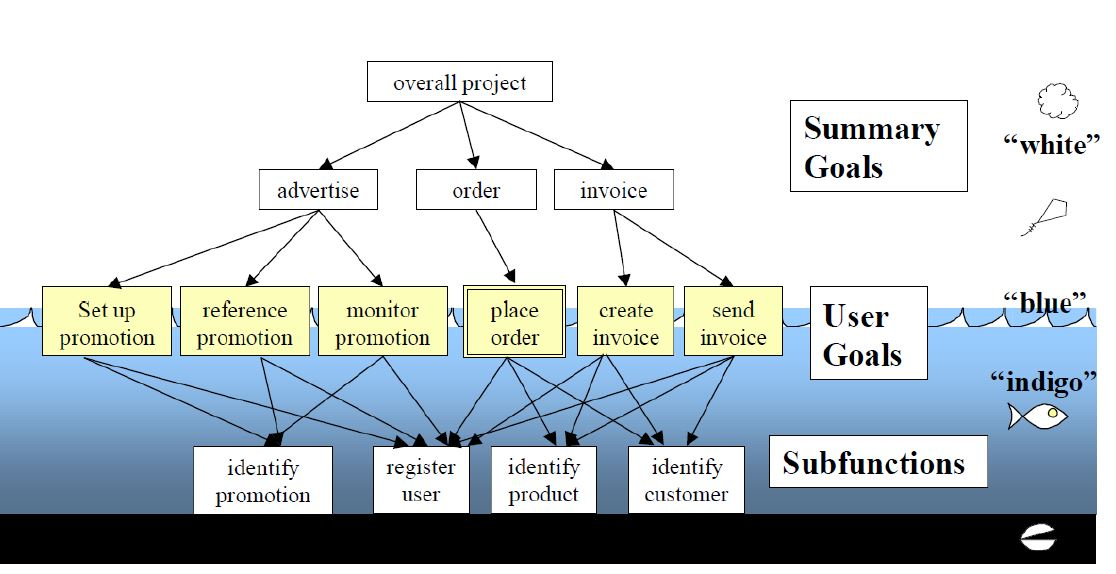
\includegraphics[width=0.9\linewidth]{fig/zielhierarchien}
\caption{Zielhierarchien}
\label{fig:zielhierarchien}
\end{figure}

Diese Hiearchien können von Top-Down oder Bottom-Up notiert werden. Nachfolgend ein Beispiel: "I want this sales contract. To do that I have to take this manager out to lunch. To do that I have to get some cash. To do that I have to withdraw money from this ATM. To do that I have to get it to accept my identity. To do that I have to get it to read my ATM card. To do that I have to find the card slot."

Die verschiedenen Farben definieren die Flughöhe. Auf Stufe weiss ist es noch sehr abstrakt. Hier haben wir im generellen die Komponenten, wie Bestellungen oder Buchungen. Basierend auf denen können auf Stufe blau die eigentlichen Benutzer-Ziele definiert werden, wie Buchung stornieren, Bestellung ausliefern. Diese basieren auf irgendwelchen Funktionen, welche wir auf Stufe indigo ansiedeln. Die Stufe schwarz ist immer sehr technisch wie beispielsweise "2 Faktor Authentfizierung". Flache Listen von Use-Cases müssen gruppiert werden. Ein Beispiel wäre nach Mitarbeiter-Funktionen.

Folgendes gilt es zu beachten, wenn die Schritte innerhalb des Use-Cases als Text verfasst werden:
\begin{itemize}
	\item Einfach formulierte Sätze beschreiben aktive Handlungen (Subjekt - Verb - Objekt).
	\item Vogelperspektive und nicht Systemsicht verwenden.
	\item Ziele entsprechen Absichten.
	\item Zeige wie der Prozess im Hinblick auf das Ziel fortschreitet.
	\item Ziel von Überprüfungen klarmachen.
	\item Wiederholungen direkt schreiben (kein Pseudocode).
\end{itemize}

Ein Vision-Statement hat folgende Inhalte: For [customer] Who [needs... or has opportunity] The [product] Is [category] That [major capability, benefit, ...] Unlike [alternative, current system, current practice] Our Product [differentiation, advantages, ...].

\section{Nichtfunktionale Anforderungen: Szenarios}

Eine Software richtet sich nicht nur nach den Anforderungen des Kunden (funktionalen Anforderungen), sondern wird auch durch Qualitätsansprüche an die Architektur (nichtfunktionale Anforderungen) beeinflusst - wie gut erfüllt das System die Bedürfnisse?. Wenn keine Nichtfunktionale Anforderungen existieren, braucht es auch keine Architektur! Nichtfunktionale Anforderungen werden einerseits durch Randbedingungen (Constraints) vorgegeben. So muss z.B. eine bestehende Softwareplattform genutzt werden oder die Zeit und Ressourcen sind zu knapp um eine verteilte Anwendung zu bauen. Die Randbedingungen schränken den Architekten bei seinen Entscheidungen also ein. 
Es gibt aber auch nichtfunktionale Anforderungen die ein Architekt sehr wohl beeinflussen kann. Dazu gehören z.B. Benutzbarkeit, Erweiterbarkeit usw. Das sind die sogenannten Qualitätsattribute. Qualitätsattribute müssen immer messbar und testbar sein. Da ein Qualitätsattribut wie eine Anforderung ist, muss auch diese SMART (siehe Abschnitt \ref{sec:funktionale-anforderungen}) sein. Die Qualitätsattribute lassen sich durch bestimmte Strukturen und Verhaltensweisen erfüllen, die von der Architektur vorgegeben werden. Funktionale Anforderungen werden erfüllt, indem bestimmte Elemente der Architektur eine Aufgabe umsetzen. Die funktionalen Anforderungen bestimmen also nicht die Architektur. 
Die Qualitätsattribute sind nicht unabhängig voneinander, weil Qualität nur indirekt messbar ist und für jeden Stakeholder etwas anderes bedeutet. Auch wenn alle funktionalen Anforderungen umgesetzt wurden, muss das nicht heissen man hat eine qualitativ hochwertige Software geschrieben. Allerdings darf man auch nicht nur auf Qualität setzen, weil dann keine Features umgesetzt werden. Deshalb sollte man immer Kompromisse bei seinen Entscheidungen eingehen.

Qualitätsattribute lassen sich in Szenarien festhalten. Ein Szenario besteht immer aus folgenden Elementen:
\begin{itemize}
	\item Quelle des Auslösers (Benutzer, Entwickler) (Stimulus Source)
	\item Auslöser / Ereignis (Stimulus)
	\item Umgebung (zur Laufzeit, während Installation) (Enviornment Artifact)
	\item Systembestandteil (z.B GUI oder Backend)
	\item Antwort / Reaktion (Response)
	\item Antwortmetrik (Wie messen wir die Antwort?) (Response Measure)
\end{itemize}

Beispielszenario:
\begin{figure}[h!]
\centering
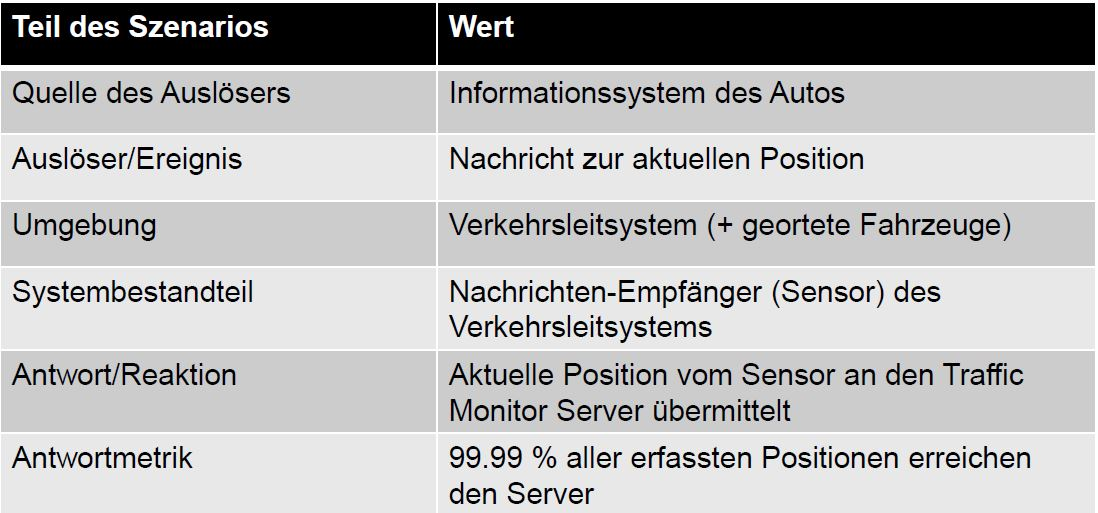
\includegraphics[width=0.7\linewidth]{fig/sample-scenario}
\caption{Beispiel-Szenario}
\label{fig:sample-scenario}
\end{figure}


Ein Qualitätsattribut lässt sich problemlos in mehrere Szenarien aufschlüsseln, damit die Anforderung detaillierter beschrieben werden kann. Hat man die Szenarien bis ins Detail ausgearbeitet, können Taktiken und Muster angewendet werden um die gewünschten Ergebnisse zu erhalten.
Nachfolgend werden einige Qualitätsattribute genauer beschrieben.

\subsection{Availability}

Funktionalitäten sind vorhanden und benutzbar wenn sie gebraucht werden. Das System muss also stabil und zuverlässig sein. Ein Ausfall sollte möglichst verhindert werden. Kommt es trotzdem zu einem Ausfall muss man das System in einer bestimmten Zeit wiederherstellen. Es können folgende Fehler auftreten (Auslöser eines Szenarios):
\begin{description}
	\item[Omission:] keine Antwort auf eine Anfrage
	\item[Crash:] Omissions treten wiederholt auf
	\item[Timing:] Response tritt zu falscher Zeit ein (zu früh, zu spät)
	\item[Response:] falscher Response des Systems
\end{description}
Diese Fehler können folgendermassen bekämpft werden:
\begin{description}
	\item[Prevention:] Einbau von Redundanz, Sicherheitsfunktionen oder Lastbegrenzungen
	\item[Detection \& Isolation:] Logging des Fehlers
	\item[Recovery:] Benachrichtigung von Benutzern und anderen Systemen, Aktionen zur Schadensbegrenzung oder einschränken der Verfügbarkeit oder Funktionalität des betroffenen Systems
\end{description}
Folgende Messwerte können zur Statistik verwendet werden:
\begin{itemize}
	\item Mean Time to Recover (MTTR)
	\item Mean Time to Failure (MTTF)
	\item Mean Time between Failure (MTBF)
\end{itemize}
\begin{figure}[h!]
\centering
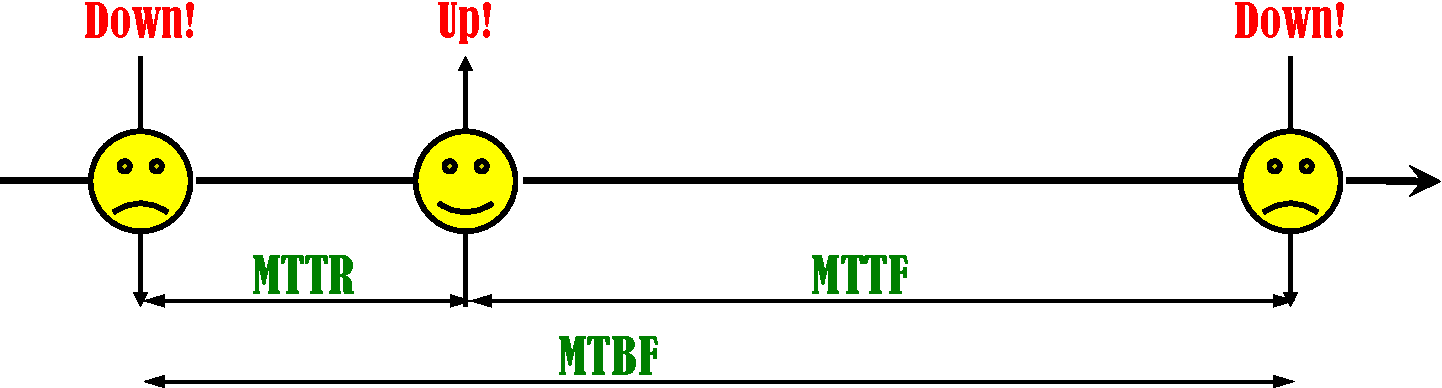
\includegraphics[width=\linewidth]{fig/mbegriffe}
\caption{M-Begriffe}
\label{fig:mbegriffe}
\end{figure}

\subsection{Interoperability}

Die Interoperabilität beschreibt den Grad in dem zwei oder mehr Systeme Information sinnvoll austauschen können. Dabei geht es um die Schnittstellen mit anderen Systemen und wie diese Systeme die Daten interpretieren.

\subsection{Modifiability}

Die Modifizierbarkeit beschreibt welche Ressourcen für eine Änderung notwendig sind und wie hoch das Risiko dafür ist. Abbildung \ref{fig:modifiability} zeigt ein Beispiel-Szenario für die Erweiterbarkeit.

\begin{figure}[h!]
\centering
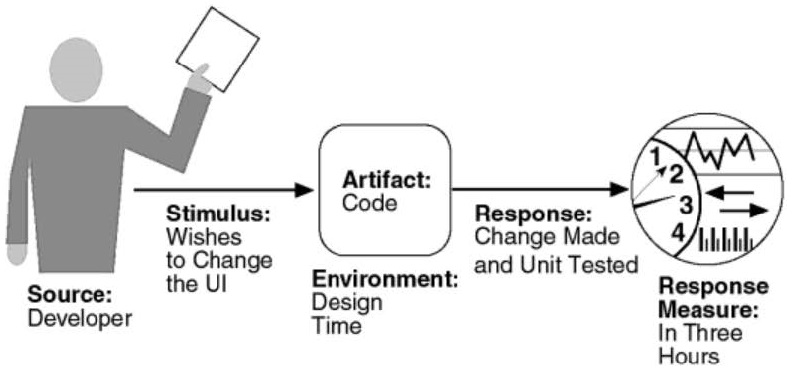
\includegraphics[width=0.7\linewidth]{fig/modifiability}
\caption{Szenario Modifiability}
\label{fig:modifiability}
\end{figure}

\subsection{Performance}

Die Performance beschreibt die Zeit in der ein System auf ein bestimmtes Ereignis reagiert. Messwerte sind Latenz (Zeit zwischen Ereignis und Reaktion), Durchsatz oder Jitter (Anzahl nicht verarbeiteter Events).

\begin{figure}[h!]
\centering
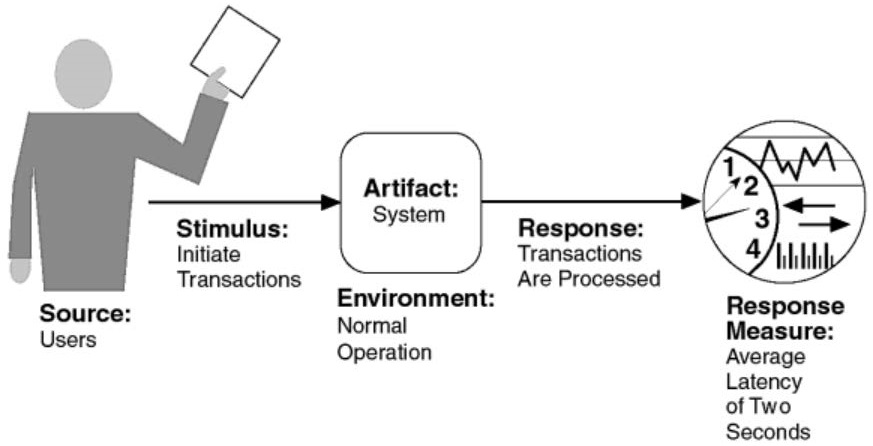
\includegraphics[width=0.7\linewidth]{fig/performance}
\caption{Szenario Performance}
\label{fig:performance}
\end{figure}

\subsection{Security}

Ein System soll Informationen vor nicht berechtigtem Zugriff schützen. Auch die Integrität der Daten muss gewährleistet sein. Darum müssen Angriffe erkannt und entsprechend darauf reagiert werden. Abbildung \ref{fig:security} zeigt ein mögliches Szenario.

\begin{figure}[h!]
\centering
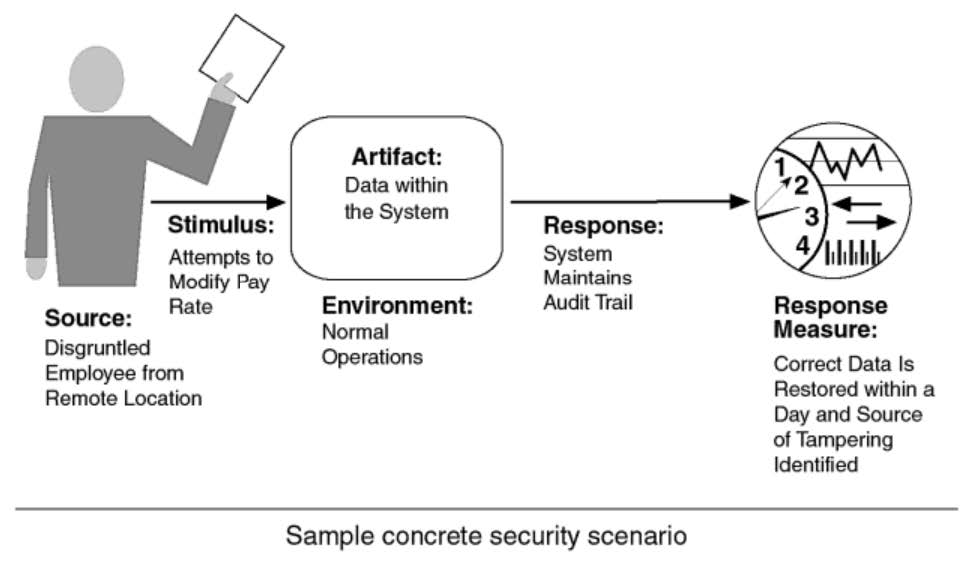
\includegraphics[width=0.7\linewidth]{fig/security}
\caption{Szenario Security}
\label{fig:security}
\end{figure}

\subsection{Testability}

Die Testbarkeit ist die Einfachheit mit der Fehler im System festgestellt werden können. Abbildung \ref{fig:testability} zeigt ein mögliches Szenario.

\begin{figure}[h!]
\centering
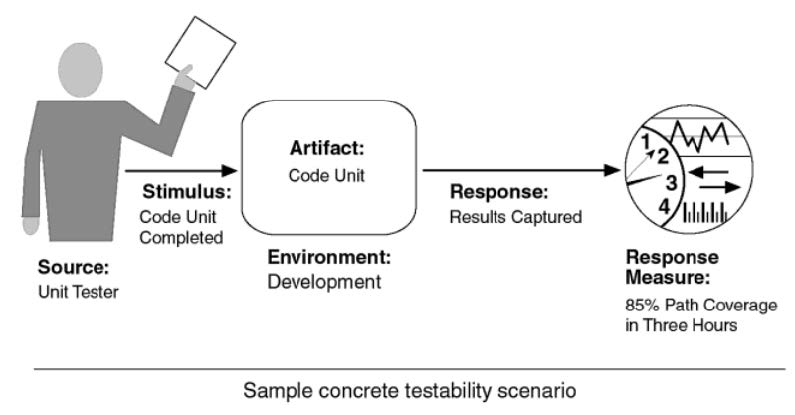
\includegraphics[width=0.7\linewidth]{fig/testability}
\caption{Szenario Testability}
\label{fig:testability}
\end{figure}

\subsection{Usability}

Mit Usability ist die Benutzerfreundlichkeit eines Systems gemeint. So soll z.B. die Einarbeitung in ein neues System nicht viel Zeit in Anspruch nehmen. Abbildung \ref{fig:usability} zeigt ein mögliches Szenario.

\begin{figure}[h!]
\centering
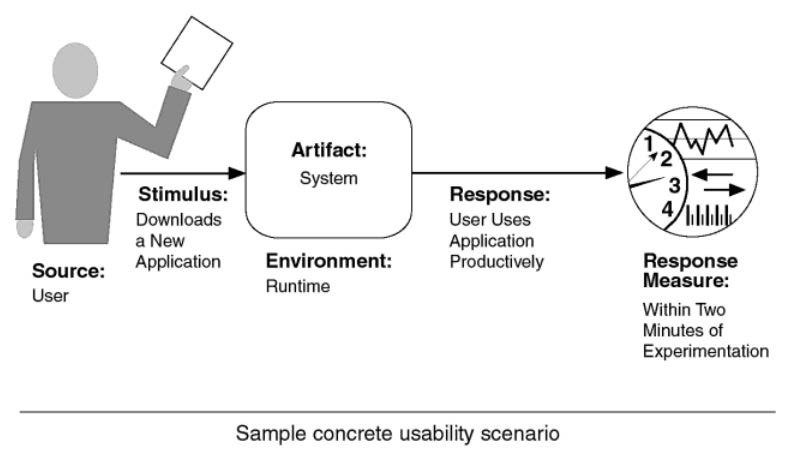
\includegraphics[width=0.7\linewidth]{fig/usability}
\caption{Szenario Usability}
\label{fig:usability}
\end{figure}

\subsection{Reusablity}

Die Wiederverwendbarkeit ist eine Eigenschaft des Systems zur Entwicklungszeit. Weisen die Komponenten hohe Wiederverwendbarkeit können Kosten gespart werden in dem viele fast gleiche Systeme gebaut werden.

\section{Prinzipien und Taktiken}
Der Architekt muss Entscheidungen treffen und diese in der Systemstruktur umsetzen. Das heisst oft, dass Kompromisse gefunden werden müssen. Grundlegend werden gute Ideen wiederverwendet und neue Ideen müssen früh validiert werden. Zudem können Prinzipien \& Taktiken angewendet und Stile \& Muster eingesetzt werden. Prinzipien sind sehr allgemeine Richtlinien wobei Stile, Taktiken und Muster detaillierte Lösungsansätze für konkrete Entwurfsentscheidungen bieten.

\subsection{Prinzipien}
Architektur-Prinzipien repräsentieren bewährte Grundsätze, die bei der Gestaltung einer Architektur zur Anwendung kommen sollten. Mit dem Ziel die Komplexität zu reduzieren und die Flexbilität sowie die Änderbarkeit zu erhöhen. Die Prinzipien sagen nichts darüber aus wie sie konkret angewendet werden! Nachfolgen einige Prinzipien:

\begin{description}
	\item[Lose Kopplung (Loose Coupling)] Jede Form der Abhängigkeit zwischen zwei Komponenten stellt eine Kopplung dar. Pro Abhängigkeit wird Erzeuger wie Verbraucher definiert. Der Verbraucher ist abhängig vom Erzeuger. Das Ziel ist es, dass der Erzeuger möglichst unabhängig vom Verbraucher geändert werden kann. Lose Kopplung erreichen wir durch Abstraktion, Separation of Concerns, Information Hiding, Messages Queues, etc.
	
	Auch das uns bekannte Hollywood-Prinzip fördert die lose Kopplung. Mittels \emph{Dependency Inversion} definieren wir die Schnittstelle mit der unserer Komponente arbeitet selbst. Andere Komponenten müssen diese Schnittstelle implementieren. Und \emph{Dependency Injection} überträgt die Verantwortung für das Erzeugen von Komponenten an ein externes Framework. Die Abhängigkeiten werden im Framework verwaltet.
	
	\item[Hohe Kohäsion (High Cohasion)] Der innere Zusammenhalt einer Komponente sollte möglichst gross sein. Eine Komponente lässt sich so leicht ändern, wenn sie alle relevanten Eigenschaften enthält um sie zu verstehen. Der Einsatz von Abstraktion, Separation of Concerns sowie Information Hiding fördert die Kohäsion.
		
	\item[Entwurf für Veränderung (Design for Change)] Vorhersehbare Änderungen architektonisch vorausplanen. Aber genauso sollen nicht vorhersehbare Änderungen auch unberücksichtigt bleiben, sonst wird man nie fertig und das Problem der zu flexibeln Architektur entsteht. Wir verwenden lose Kopplung, Abstraktion, Modularität, Seperation of Concern und Information Hiding.
	
	\item[Trennung der Verantwortlichkeiten (Separation of Concerns)] Die Verantwortlichkeiten von Komponenten sind genau zu definieren. Die Komponenten soll nur genau das Eine tun, dafür vollständig! Verschiedene Aspekte von Probleme sind zu trennen. Für die Zerlegung gibt es mehrere Ansätze: Anforderungen, Software-System in eine Struktur von Systembausteinen, komplexe Architektur-Beschreibung in Sichten, organisatorische Verantwortlichkeiten, Prozesse der Architektur-Erstellung in Teilprozesse.
	Mittels Modularität kann die Zerlegung auf der Basis auf den funktionalen Anforderungen erfolgen. Beispielsweise: Benutzerschnittstellen, Bestellabwicklung, Datenbankzugriff, etc. Zudem kann es auch Sinn machen, wenn wir die technischen Schichten weiter mittels fachlichen Schichten trennen (siehe Bild \ref{fig:schichten-architektur})
	
	\begin{figure}[h!]
	\centering
	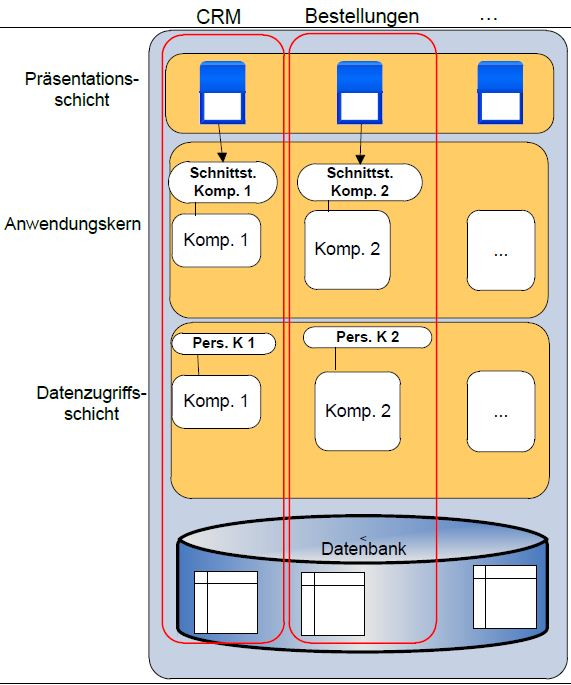
\includegraphics[width=0.6\linewidth]{fig/schichten-architektur}
	\caption{Schichten-Architektur: Technische wie fachliche Trennung}
	\label{fig:schichten-architektur}
	\end{figure}

	\item[Geheimhaltung (Information Hiding)] Alles verbergen, was nicht benötigt wird. So entstehen keine unnötigen Abhängigkeiten. In der OOP alle Daten als privat markieren. Ein Fassade Pattern kann dazu dienen, alles andere zu verstecken. Bei der Schichtung kann die darüberliegende Schicht nur auf die darunterliegende Schicht zugreifen.
	
	\item[Abstraktion] Bei der Abstraktion werden wichtige Aspekte identifiziert und unwichtige Details vernachlässigt. Es ist schlussendlich ein Spezialfall der Geheimhaltung. Das wichtigste Teilprinzip nennt sich \emph{Schnittstellensabstraktion}, denn erst durch die Beziehungen der Bausteine eines Systems untereinander kommt eine Architektur wirklich zum Tragen. Mittels Geheimhaltung und Abstraktion wird die Portabilität der Architektur gestärkt (Plattform-Unabhängigkeit). Folgendes noch zur Schnittstellensabstraktion:
	
	\begin{itemize}
		\item Alle Schnittstellen werden explizit angegeben, Kommunikation nach aussen nur über diese Schnittstellen möglich.
		\item Trennung von Schnittstelle und Implementierung.
		\item Liskov-Substitution: Erbende Klassen durch die Schnittstelle der vererbende Klasse aufrufbar.
		\item Schnittstelle-Segregation: Ein Klient soll nie auf einer Schnittstelle basieren, die er nie benutzt. Komplexe Schnittstellen in mehrere einzelne Schnittstellen auftrennen.
		\item Design by Contract: Vor-, Nachbediengungen sowie Invarianten einer Schnittstelle explizit angeben.
	\end{itemize}
		
	\item[Modularität] Zerlegung eines Systems in definierte Systembausteine, deren funktionale Verantwortlichkeiten klar abgegrenzt sind. Systembausteine leicht austauschbar und in sich abgeschlossen. Diese sind überschaubar, verstehbar, leicht wartbar und wiederverwendbar.Einfache und stabile architektonische Beziehungen. Kombination von Abstraktion, Separation of Concerns und Information Hiding.
	
	Bausteine sollen offen für Veränderungen sein (Entwurf für Veränderung) und geschlossen für die Nutzung der internen Details durch andere Systembausteine (Abstraktionen, Geheimhaltung).
	
	\item[Rückverfolgbarkeit (Traceability)] Architektonische Strukturen und Entscheidungen durchgängig von den Anforderungen über die Modelle zum Code verfolgbar. Dies soll die Verständlichkeit der Architektur erhöhen. Wichtig ist, dass einheitliche Namenskonventionen verwendet werden. Leichter verstehbare Strukturen sind unabhängiger voneinander und leichter zu ändern.
	
	\item[Selbstdokumentation] Jede Information über einen Systembaustein sollte zum Bestandteil des Systembausteins selbst gemacht werden. In der Realität laufen Dokumentation und Software jedoch schnell auseinander. Nach Möglichkeit soll die Dokumentation genau dort gemacht werden, wo die Software entsteht. Unterstützt so auch die Rückverfolgbarkeit.
	
	\item[Inkrementalität] Inkrementalität bedeutet, das Prinzip der Trennung der Verantwortlichkeiten auf die Entwicklungsschritte bei der Systementwicklung anzuwenden. Früh erste Version ausliefern, früh die Meinung von Benutzer einholen, neue Funktionen nur schrittweise einführen (piecemeal growth).
	
\end{description}

Bild \ref{fig:abhangigkeiten-prinzipien} zeigt die Beziehung der einzelnen Prinzipien untereinander.

\begin{figure}[h!]
	\centering
	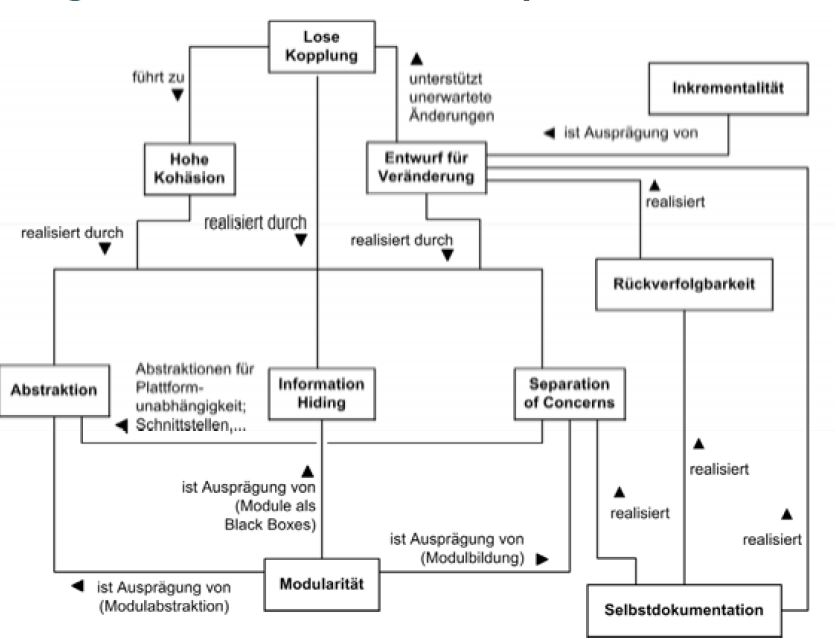
\includegraphics[width=0.6\linewidth]{fig/abhaengigkeiten-prinzipien}
	\caption{Abhängigkeiten von Prinzipien}
	\label{fig:abhangigkeiten-prinzipien}
\end{figure}

\subsection{Taktiken}
\emph{There are many was to do design badly, and just a few ways to do it well.} Taktiken definieren Richtlinien zur Verbesserung der Architektur. Sie sollen als Hilfe für den Architekten dienen eine erste Idee zu einem Entwurfsproblem zu erhalten. \textbf{Eine Taktik ist eine Entwurfsentscheidung, die Einfluss nimmt auf die Realisierung der Reaktion eines Qualitätsattributszenarios.}. Bestimmt somit mit welchem Response das System auf einen Stimulus eines Qualitätsattributs reagiert. Dabei werden keine Kompromisse (Trade-offs) berücksichtigt.

Für alle Taktiken kann man sicher immer folgende Entscheidungen überlegen (7 Arten von Entscheidungen):
\begin{itemize}
	\item Zuordnung von Verantwortlichkeiten: Welche Elemente im System sind für welche Funktionen und Qualitätsattribute verantwortlich?
	\item Koordinationsmodel: Wie interagieren welche Elemente? Welche dürfen nicht interagieren?
	\item Datenmodell (inkl. Datenhaltung)
	\item Resourcenmanagement: Wie werden welche Resourcen "gemanaged", "geshared"? Welcher Resourcenbedarf besteht?.
	\item Zuordnungen von Architekturelementen (mapping): Innerhalb der Architektur: z.B. Module und Laufzeit-prozesse oder innerhalb Umgebung: z.B. Prozesse und CPU Elemente.
	\item Binding time decisions: Variabilität in der Architektur.
	\item Technologiewahl: Vorgegeben als Constraint oder Wahl des Architekten
\end{itemize}


\begin{description}
	\item[Taktiken für Verfügbarkeit] Die Verfügbarkeit wird durch Failures (Service kann nicht mehr erbracht werden) und Faults (Mangel, Defekt, kann ein Failure werden) eingeschränkt. Taktiken für die Verfügbarkeit zielen darauf ab, dass das System Faults abfangen kann, dass kein Failure entsteht.
	
	\begin{figure}[h!]
	\centering
	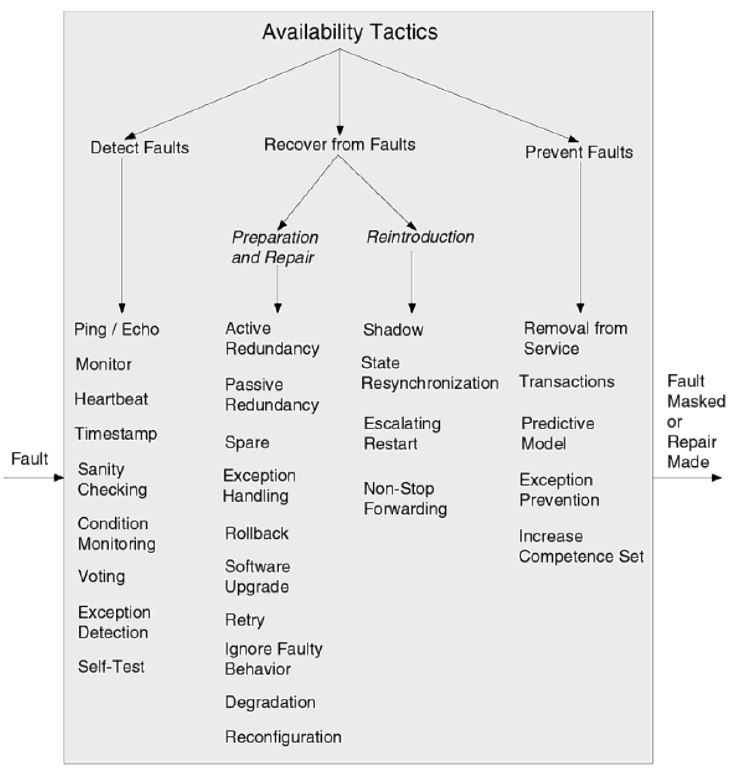
\includegraphics[width=0.7\linewidth]{fig/tactic-availability}
	\caption{Availability-Taktiken}
	\label{fig:tactic-availability}
	\end{figure}
	
	\item[Taktiken für Modifiability]
	\begin{figure}[h!]
	\centering
	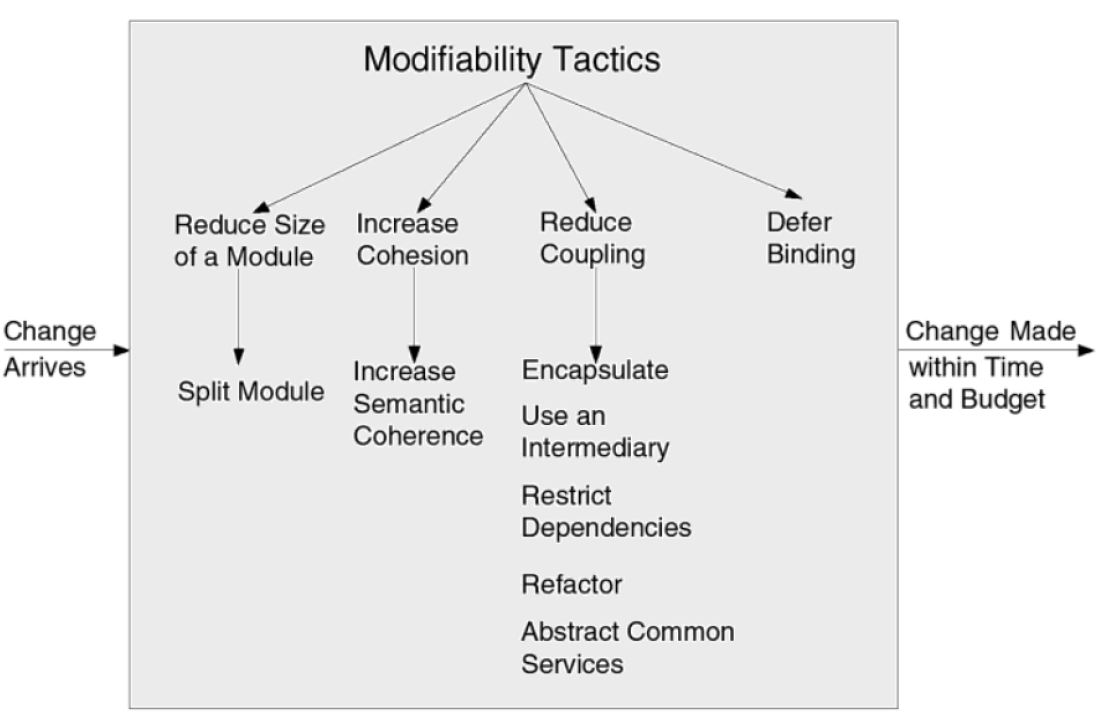
\includegraphics[width=0.7\linewidth]{fig/tactic-modifability}
	\caption{Taktiken für Modifiability}
	\label{fig:tactic-modifability}
	\end{figure}

	\item[Taktiken für Performance]
	\begin{figure}[h!]
	\centering
	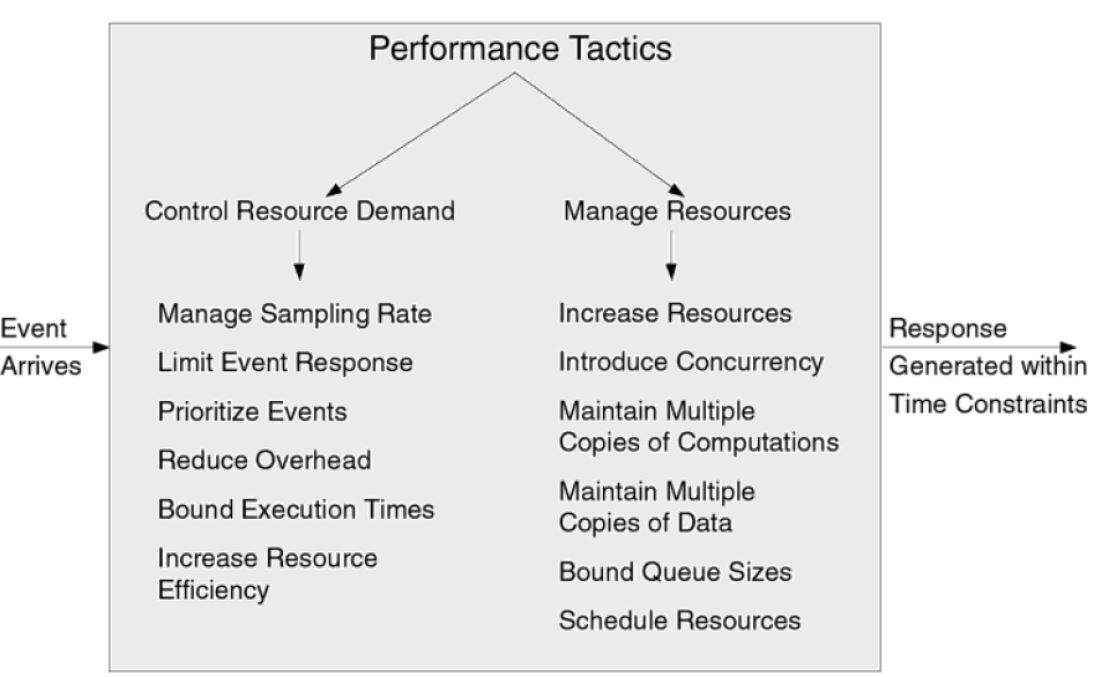
\includegraphics[width=0.7\linewidth]{fig/tactic-performance}
	\caption{Taktiken für Performance}
	\label{fig:tactic-performance}
	\end{figure}
	
\end{description}

\subsection{Systemidee entwickeln}
Eine erste Systemidee kann entwickelt werden, wenn wir die Prinzipien und Taktiken auf das Entwurfsproblem angewendet werden. Es ist ein kreativer Prozess, es gibt mehr als eine Lösung, Kompromisse finden, die richtigen Fragen stellen und bewährte Lösungen wiederverwenden.

Architektur heisst Entscheidungen treffen: \emph{A software system's architecture is the set of principal design decisions made about the system}. Welches immer auf Kompromisse basiert. Es können nie alle Qualitätsattribute zu 100 Prozent erfüllt werden - trade off finden!

\begin{figure}[h!]
\centering
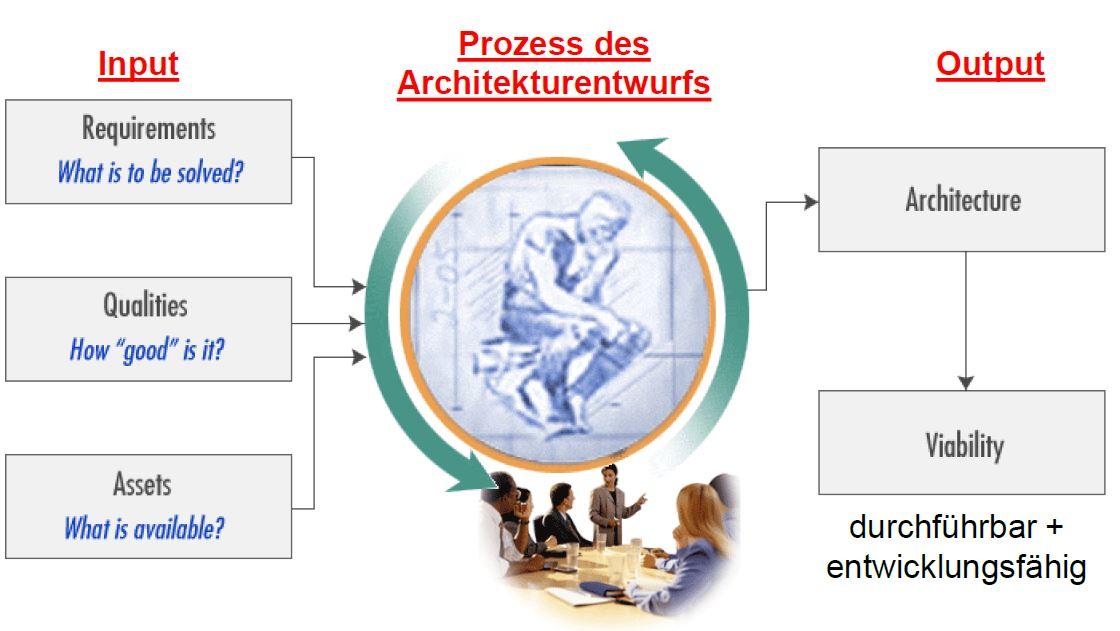
\includegraphics[width=0.7\linewidth]{fig/architectural-thinking}
\caption{Architectural Thinking}
\label{fig:architectural-thinking}
\end{figure}

\subsection{Domain-Driven-Design}
Genauso wichtig wie die vielen technischen Komponenten ist die Fachdomäne (Domain-Driven-Design). Ein stabiles und akzeptiertes Domänenmodell ist fundamental. Als Basisbausteine dienen: Entities (unverändlichere Idendität, klarer Lebenszyklus, meist persistent), Value Objects (Beschreiben Zustand anderer Objekte) und Services (Abläufe, Prozesse).

\begin{figure}[h!]
\centering
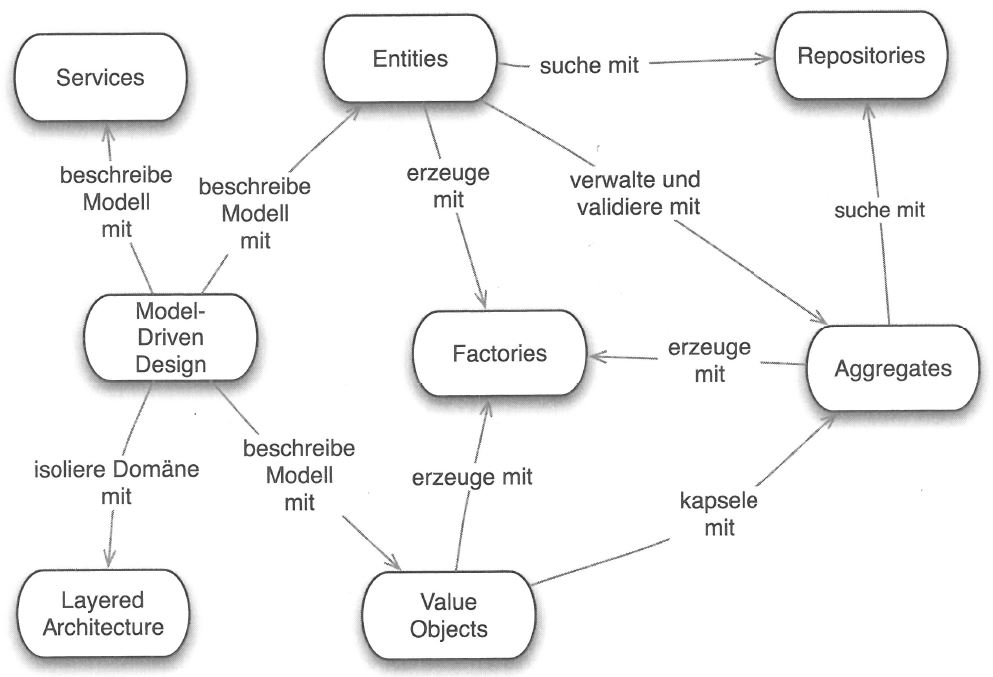
\includegraphics[width=0.7\linewidth]{fig/domain-driven-design}
\caption{Domain-Driven-Design}
\label{fig:domain-driven-design}
\end{figure}

\subsection{Zentralisierung vs. Dezentralisierung}
Immer wieder stellt sich der Architekt die Frage ob er einen Aspekt in der Architektur in einem Baustein bündeln oder auf mehrere Bausteine verteilen soll? Im Vordergrund stehen Einfachheit, Schlichtheit und Verständlichkeit. Die Zentralisierung bietet folgende Vorteile: Hohe Datensicherheit, leichte Systemintegraton, Ausfallsicherheit leichter zu gewährleisten, einfacher zu administrieren. Es besteht jedoch die Gefahr von Monolithen, eventuell hohe Hardware-Kosten, Hersteller- und Technologie Abhängigkeiten. Die Dezentralisierung bietet tendenziell niedrige Hardware-Kosten, höhere Flexibilität und kleinere Komponenten. Jedoch ist der Integrationsaufwand höher, Abhängigkeit von Netz sowie schwieriger zu administrieren.

\subsection{Empfehlungen für den Entwurf von Systemstrukturen}
\begin{itemize}
	\item Komponentenfunktionalität ist wohldefiniert und setzt Geheimnisprinzip und Trennung der Verantwortlichkeiten um.
	\item Schnittstellen sind wohldefiniert und "verstecken" Veränderungen.
	\item Entwicklungsteams können Komponenten unabhängig voneinander umsetzen auf der Basis der Schnittstellen-definitionen.
	\item Taktiken und Muster werden eingesetzt.
	\item Architektur darf niemals von einem bestimmten Produkt/Tool abhängen.
	\item Daten produzierende und Daten konsumierende Module sind klar voneinander getrennt.
	\item Es muss keine 1-1 Beziehung zwischen (Entwicklungs)-modulen und (Runtime)-Komponenten geben.
	\item Prozesse sollten leicht änderbar sein, ggf. zur Laufzeit.
	\item Nur wenige Arten von Interaktion sollten im System vorhanden sein.
	\item Die gleiche Art von Interaktion sollte gleich umgesetzt werden.
	\item Ressourcenkonflikte sind eingegrenzt und ihre Auflösung ist klar definiert.
\end{itemize}

\subsection{Empfehlungen für den Prozess des Entwurfs}
\begin{itemize}
	\item Die Architektur sollte von einem einzelnen Architekten oder einem kleinen Team entworfen worden sein.
	\item Es sollte eine enge und produktive Beziehung zwischen dem Architektenteam und dem Entwicklungsteam bestehen.
	\item Entwürfe basieren auf einer aktuellen priorisierten Liste der Qualitätsattribute.
	\item Sichten für die wichtigsten Stakeholder werden erstellt.
	\item Evaluation der Entwürfe passiert frühzeitig u. wird bei Änderungen wiederholt.
	\item Die Architektur untersützt einen inkrementellen Entwicklungsprozess.
	\item Conway's Law: Architektur = Team Organisation
\end{itemize}

It states that organizations which design systems ... are constrained to produce designs which are copies of the communication structures of these organizations — M. Conway.

\section{Stile und Muster}

\subsection{Stile}

Ein Architektur-Stil beschreibt ein Muster zur strukturellen Organisation einer Familie von Systemen. Diese fundamentale Struktur beschreibt folgende Eigenschaften eines Software-Systems:
\begin{itemize}
	\item Die Komponententypen und welche Funktionen diese zur Laufzeit erfüllen.
	\item Die topologische Anordnung dieser Komponenten.
	\item Die Konnektoren, welche die Kommunikation und Koordination zwischen den Komponenten regeln.
	\item Eine Menge von semantischen Einschränkungen, die bestimmen, wie Komponenten und Konnektoren miteinander verbunden werden können.
\end{itemize}
Es haben sich folgende Stil herausgebildet, die in den nachfolgenden Abschnitten beschrieben werden:
\begin{itemize}
	\item Schichten (Layers, Tiers)
	\item Pipes \& Filters
	\item Verteilte Systeme (Client/Server, Peer-to-Peer)
	\item Blackboard
	\item Service-orientierte Architekturen (SOA)
\end{itemize}

\subsubsection{Schichten}

Ein System wird in Schichten aufgeteilt, deren Elemente einen ähnlichen Abstraktionsgrad besitzen. Eine Schicht benutzt nur die Services, welche von der direkt darunterliegenden Schicht zur Verfügung gestellt werden. Das Überspringen einer Schicht zerstört die Architektur. Schichten haben folgende Vor- bzw. Nachteile:
\begin{itemize}
	\item[+] Leicht verständliches Strukturkonzept
	\item[+] Minimiert Abhängigkeiten zwischen Komponenten
	\item[+] Schichten sind voneinander unabhängig in Erstellung und Betrieb
	\item[+] Änderungen in einer Schicht können maximal eine andere Schicht betreffen
	\item[--] Kann die Performance eines Systems beeinträchtigen, wenn Anfragen durch mehrere Schichten weitergereicht werden müssen
	\item[--] Änderungen im Datenmodell können alle Schichten betreffen (Datenverwaltung, Applikation, Präsentation)
\end{itemize}

\subsubsection{Pipes \& Filters}

Bei diesem Stil werden Verarbeitungseinheiten (Filter) hintereinander geschaltet und durch Datenkanäle (Pipes) verbunden. Jeder Filter gibt sein Ergebnis direkt an den nächsten Filter weiter. Pipes sind keine eigenen Komponenten in der Architektur sondern dienen rein als Konnektoren. Es sind verschiedene Koordinationsmodelle denkbar, so kann die Steuerung zentral oder dezentral sein, die Pipes aktiv oder passiv und die Datenübergabe komplett, stückchenweise oder zeitversetzt geschehen. Pipes \& Filters bieten folgende Vor- bzw. Nachteile:
\begin{itemize}
	\item[+] Einfache Implementierung
	\item[+] Klar verständliche Struktur
	\item[+] Klar strukturierte Abläufe
	\item[+] Mächtige Pipes können entscheiden, an welche Instanz eines Filters (Load balancing) oder an welchen Filter (Kapselung) sie die Daten weitergeben
	\item[--] Filter kennen einander nicht (Folgefehler können von ihnen nicht behandelt werden)
	\item[--] Konfiguration der Verarbeitungskette kann schwierig sein
	\item[--] Filter können nur über Daten kommunizieren (Gesamte Verarbeitungsinformation muss in den Daten oder der zentralen Steuerung enthalten sein)
\end{itemize}

\subsubsection{Verteilte Systeme}

Verteilte Systeme können entweder als \textbf{Client/Server} oder als \textbf{P2P-Netzwerk} betrieben werden. Der Client wird als Applikation lokal betrieben und kommuniziert über ein Anfrage-Antwort-Schema mit dem zentral zur Verfügung gestellten Server. Dabei kann auf dem Client zwischen Thin Client (z.B. Gmail) und Rich Client (z.B. Outlook) unterschieden werden. Der Client/Server-Stil bietet folgende Vor- bzw. Nachteile:
\begin{itemize}
	\item[+] Zentralisierung wichtiger, rechenintensiver oder sensibler Berechnungen im Server
	\item[+] Thin Clients einfach in Verteilung und Wartung
	\item[+] Rich Clients oft bei Server-Ausfall noch verwendbar
	\item[--] Netzbelastung hoch (besonders bei Thin Clients)
	\item[--] Verteilung der Funktionalität nicht immer einfach
	\item[--] Grenzen der Skalierung bei sehr hohen Clientzahlen
\end{itemize}

Bei einem P2P-Netzwerk kommunizieren verteilte Komponenten (Peers), die sowohl die Rolle von Clients als auch Servern wahrnehmen und sich Ressourcen teilen. Die Komponenten sind über eine Art Konnektor (z.B. Internet) miteinander verbunden. Bei einem P2P-Netzwerk gibt es keine zentrale Kontrolle, es kann also jeder Peer mit jedem Peer kommunizieren. Die Lokalisierung kann durch dezentrale Kommunikation (Peers tauschen untereinander ihre Listen bekannter Peers aus) oder durch einen zentralen Service realisiert werden. Das P2P-Netzwerk hat folgende Vor- bzw. Nachteile:
\begin{itemize}
	\item[+] Hohe Ausfallsicherheit (kein single point of failure)
	\item[+] Rechenintensive Aufgaben können verteilt werden
	\item[--] Auffinden und Erkennen von Peers in grossen Netzen
	\item[--] Potentielle Gefahr des Zerfalls des P2P Netzes (Nur bestimmte Gruppen von Peers kennen sich)
	\item[--] Fehlerbehandlung (Wer reagiert, wenn ein Peer seine Aufgaben falsch löst?)
	\item[--] Keine garantierten Antwortzeiten
\end{itemize}

\subsubsection{Blackboard}

Der Blackboard-Stil kommt ursprünglich aus der Künstlichen Intelligenz zur Lösung komplexer Probleme, für die kein deterministisches Lösungsverfahren existiert. An der Problemlösung arbeiten mehrere unabhängige Programme welche ein Blackboard als zentralen Datenspeicher verwenden. Die Programme kommunizieren also nicht untereinander sondern nur über ein zentrales Blackboard. Eine zentrale Steuerungskomponente bewertet den Lösungsfortschritt auf dem Blackboard und aktiviert die verfügbaren Programme. Das Blackboard hat folgende Vor- bzw. Nachteile:
\begin{itemize}
	\item[+] Einfache Integration komplexer Systeme
	\item[+] Parallelisierung der Berechnungen möglich
	\item[+] Moderne Variante: Tuple Space
	\item[--] Keine Garantie der Lösungsfindung
	\item[--] Finden der richtigen Kontrollstrategie ist schwierig
	\item[--] Keine garantierten Antwortzeiten
\end{itemize}

\subsubsection{SOA}

SOA wurde mega gehypt und nun machen sich alle darüber lustig und verwenden stattdessen Microservices, welche nun alle Probleme dieser Welt lösen. SOA versucht eine Spezifikation der Service, Datenformate und Kommunikationsprotokolle zu erreichen. Die Applikation wird dann als Orchestrierung von verschiedenen Services zur Erreichung der Geschäftsziele entworfen. Ein Service Consumer verwendet über ein Integration Layer (Middleware) ein Service eines Service Providers. Services tauche in allen Schichten auf und kommunizieren über einen zentralen Enterprise Service Bus. So gibt es natürlich Services für das Business aber auch für die Entwicklung oder die Infrastruktur. Service-orientierte Systeme sollten modular, verteilbar, auffindbar, austauschbar und wiederverwendbar sein. Wichtig dabei ist eine saubere Trennung der Verantwortlichkeiten und lose Kopplung. Ohne eine zentrale Stelle (SOA Governance) welche ein Überblick über das Ganze behält, wird jede Umsetzung von SOA scheitern. SOA bietet folgende Vor- bzw. Nachteile:
\begin{itemize}
	\item[+] descriptionSehr flexible Architekturform mit einfachem Grundmodell
	\item[+] Vielzahl von ausgereiften Standards
	\item[+] Verbindung von Business und IT
	\item[+] Voraussetzung für Cloud, Mashups usw.
	\item[--] Zusätzliche Komplexität wegen offener, dezentralisierter Systeme	
	\item[+] Vielzahl schwieriger Fragestellungen (Service design, Interoperabilität, Standards)
\end{itemize}

\begin{figure}[h!]
\centering
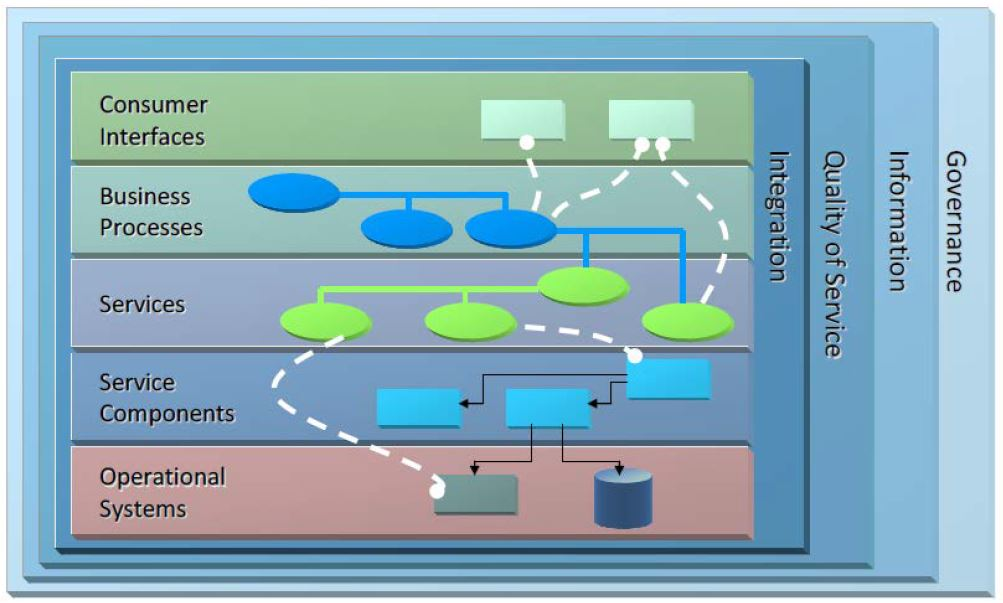
\includegraphics[width=0.7\linewidth]{fig/soa-reference-architecture}
\caption{SOA Reference Architecture}
\label{fig:soa-reference-architecture}
\end{figure}


\subsection{Muster}

Ein Muster in der Software-Architektur beschreibt ein generisches, well-proven Schema, welches in spezifischen Kontext genutzt werden kann. Ein Architekturmuster erfindet man nicht einfach, sondern erkennt man mithilfe von Erfahrungen aus der Praxis. Ein Muster setzt mehrere Taktiken um, aber macht auch immer einen Kompromiss zwischen mehreren Qualitätsattributen. Die Aufgabe des Architekten ist das richtige Muster anhand des Kontexts und den Rahmenbedingungen zu finden. Er muss sich auch genau überlegen, wie der Kompromiss des Musters die eigene Lösung beeinflusst. Ein Muster wird immer durch den Kontext, das Problem und die Lösung beschrieben.

Um ein System oder eine Komponente in eine bestehende Umgebung einzubinden existieren folgende vier Patterns (Enterprise Integration Patterns, Technologie unabhängig):
\begin{itemize}
	\item File Transfer
	\item Shared Database
	\item Remote Procedure Invocation (RPC)
	\item Messaging
\end{itemize}
Diese Patterns werden nachfolgend detailliert beschrieben:

\subsubsection{File Transfer}

Beim File Transfer wird eine Datei irgendwo zentral abgelegt, damit beide Applikationen drauf Zugriff haben. Dabei wird das Dateiformat und der Zeitintervall, in denen die Datei erzeugt und konsumiert wird, untereinander vereinbart. Dieses Muster bietet folgende Vor- bzw. Nachteile:
\begin{itemize}
	\item[+] Dateien als universelles Speichermedium
	\item[+] Minimale Anforderungen an Hardware/Software
	\item[+] Keine Kenntnisse der Applikation notwendig für Integration
	\item[+] Keine weitergehenden Abhängigkeiten zwischen integrierten Applikationen	
	\item[--] Synchronisation der Daten kann bei Änderungen schnell verloren gehen	
	\item[--] Ungeeignet für den sehr häufigen Austausch kleinerer Datenmengen (Dateimanagementproblem)
\end{itemize}

\subsubsection{Shared Database}

Bei diesem Muster wird eine Datenbank zwischen verschiedenen Applikationen geteilt. Dadurch werden die Daten konsistent und in einem einheitlichen Datenformat über die Anwendungen ausgetauscht. Die Veränderung der Daten ist über Datenbanktransaktionen gesichert. Die Shared Database bietet folgende Vor- bzw. Nachteile:
\begin{itemize}
	\item[+] Unterstützung von Datenbankstandards in allen Entwicklungsumgebungen
	\item[+] Synchronisation der Daten gesichert
	\item[--] Applikationen müssen an Datenformate angepasst werden (Adapter, Transformationen)
	\item[--] Einigung aller Applikationen auf ein einheitliches Format
	\item[--] Externe Applikationen arbeiten oft nur mit ihren eigenen Formaten (Bedarf nach zusätzlichen Adaptern)
	\item[--] Datenbank als potentieller single point of failure für alle Applikationen
	\item[--] Performanzprobleme
\end{itemize}

\subsubsection{Remote Procedure Invocation}

Beim RPC-Muster werden Methoden auf entfernten Anwendungen aufgerufen. Dabei werden die Daten zu einer Funktionalität gekoppelt. Eine Applikation wird als Komponente gekapselt, welche ihre Funktionalität über eine Schnittstelle anderen Applikationen zur Verfügung stellt. Dieses Muster bietet folgende Vor- bzw. Nachteile:
\begin{itemize}
	\item[+] Applikationen können interne Datenformate ändern
	\item[+] Unterschiedliche Schnittstellen können bereitgestellt werden
	\item[+] Einfaches Entwicklungskonzept ("Prozeduraufruf")
	\item[--] Abstimmung und Änderung von Schnittstellen über mehrere Applikationsgrenzen kann schwierig sein
	\item[--] Aufrechterhalten von veralteten Schnittstellen
	\item[--] Performanz- und Zuverlässigkeitsprobleme von Remote Aufrufen ("remote" <> "local")
	\item[--] Enge Kopplung der Applikationen ("growing knot")
\end{itemize}

\subsubsection{Messaging}

Durch Messaging wird eine lose Kopplung unter den einzelnen Systemen erreicht. Dabei wird zwischen synchroner, asynchroner und Publish-Subscribe Kommunikationsstilen unterschieden. Messaging bietet folgende Vor- bzw. Nachteile:
\begin{itemize}
	\item[+] Flexibelste Integrationslösung
	\item[+] Unterstützung durch zahlreiche Technologien
	\item[+] Transformation und Management der Daten innerhalb der Messaging Middleware und nicht in der Applikation
	\item[--] Asynchrones Design von Applikationsfunktionen nicht immer einfach
	\item[--] Testen und Debugging schwieriger
	\item[--] Flexibilität führt zu zahlreichen Folgefragen, die gelöst werden müssen
\end{itemize}

\section{Sichten, Architekturentscheidungen und Dokumentation}

\subsection{Sichten}

Eine Sicht stellt ein vollständiges System aus dem Blickwinkel einer Menge von zusammenhängenden Interessen heraus dar. Warum benötigten wir überhaupt Sichten?

\begin{itemize}
	\item Moderne Software ist oft zu komplex, um sie als Gesamtheit anschauen und verstehen zu können.
	\item Wir müssen unsere Aufmerksamkeit zu jedem Zeitpunkt auf einen (oder wenige) Teile der Systemstruktur lenken.
	\item Um problemlos kommunizieren zu können, müssen wir klar machen, welche Strukturen (oder auch Verhalten) wir jetzt diskutieren.
\end{itemize}

Zusammenfassend dient eine Sicht um eine Struktur darzustellen - sie sichtbar zu machen. Architekten entwerfen Strukturen und dokumentieren diese Strukturen durch Sichten. Gute Sichten sind:

\begin{itemize}
	\item Bedarfsgerecht
	\item So wenig Formalismus wie möglich, so viel wie nötig!
	\item Umfang der Sicht am Risiko orientiert
	\item Top-down arbeiten und Sichten weiter verfeinern
	\item Wenn die von uns intendierte Botschaften korrekt beim Empfänger angelangt.
\end{itemize}

Die Sichten sind das Resultat aus dem Entwurf und sind fundamental für das Kommunizieren der Architektur. Da es unterschiedliche Beteiligte gibt, welche unterschiedliche Brillen tragen, brauchen wir unterschiedliche Sichten.

Es gibt unterschiedlichen Sichtenmodelle. Sowohl Kruchten wie auch Starke haben eigene Modelle definiert. Beide bestehen grundsätzlich aus der Kontext-, der Laufzeit-, der Baustein- und der Verteilungssicht. Nach Kruchten gibt es noch die Szenarios.

\begin{description}
	\item[Kontextsicht] Dient als Übersichtsdiagramm zum Umfeld des Systems. Es dient für die Ressourcenplanung und fürs Risikomanagement. Darauf kann die Anzahl \& Art der Schnittstellen nach aussen, der Abhängigkeiten der Umsystemen sowie die beteiligten Stakeholder erkennen.
	
	Best-Practice: Zeichne dein System als Kasten und gib diesem einen Namen. Zeichne Umsysteme als Kasten und Rollen als Personen. Verknüpfe die Personen und Systeme mit deinem System und schreibe, welche Daten ausgetauscht werden. Achtung: Use Case ist kein Kontextdiagramm. Die Abhängigkeiten, welche die Umsysteme gegenseitig haben, interessieren eigentlich nicht.
	
	\item[Bausteinsicht] Die Bausteinsicht soll aufzeigen, wie das System intern aufgebaut ist. Es ist von statischen Strukturen wie Subsysteme, Komponenten und deren Schnittstellen die Rede.
	
	In der Regeln arbeiten wir Top-Down. Die letzte Verfeinerungsstufe ist der Quellcode selbst. Es soll den Projektleiter und Auftraggeber unterstützen. Dient ideal um Arbeitspakte zuzuteilen und ist allgemein die Referenz für die Entwickler.
	
	In UML können wir Klassendiagramme, Packetdiagramme oder Komponentendiagramme verwenden.
	
	\item[Laufzeitsicht] Im Zentrum stehen die dynamischen Strukturen und Abläufe. Welche Bausteine existieren zur Laufzeit? Wie wirken diese zusammen?
	
	In UML würden wir Aktivitätsdiagramme verwenden. Aber wir verwenden BPMN. Auf technischer Ebene kommen Sequenzdiagramm zum Einsatz.
	
	\item[Verteilungssicht] In welcher Umgebung läuft das System? Systeme aus Betreibersicht. Verteilung des System auf die physischen Systeme (Hardware, Netzwerk, Rechner, Prozessoren, Protokolle, etc.). In UML ist das Verteilungsdiagramm die erste Wahl.
\end{description}

Meine persönliche Empfehlung ist eine Datensicht. Mit einem einfachen konzeptuellen Datenmodell kann die Fachdomäne schnell verstanden werden. Zudem haben wir die Security-Sicht sowie User Experience nicht behandelt.

\subsection{Architektur-Ebenen}

Ein Architekt bewegt sich auf unterschiedlichen Architektur-Ebenen. Er muss sich bewusst sein, auf welcher Ebene er sich aktuell befindet und was seine Entscheidung auf der Ebene bewirken. Es wirken unterschiedliche Kräfte auf die Architektur. Die Bausteinebene wird von der Systemebene beeinflusst und auf die Systemebene wirken die Kräfte der Organisationsebene (Definition nach Vogel).

\begin{figure}[h!]
\centering
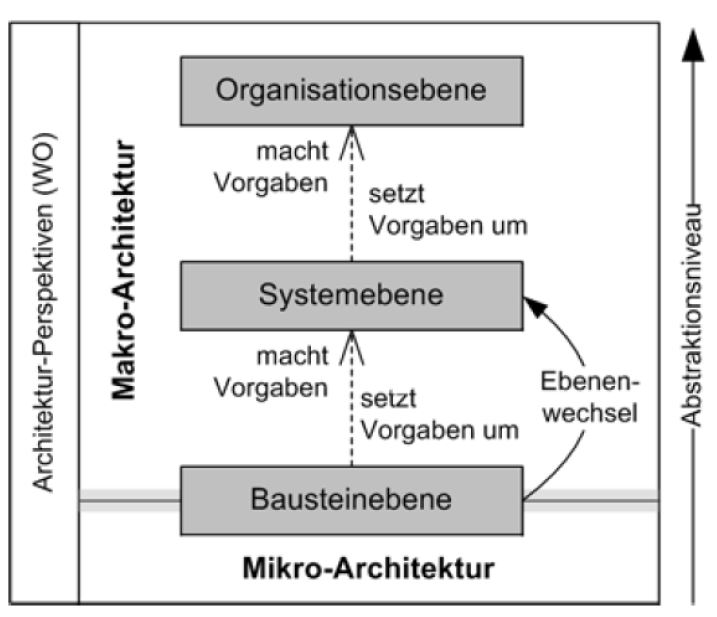
\includegraphics[width=0.5\linewidth]{fig/architekur-ebenen}
\caption{Architektur-Ebenen}
\label{fig:architekur-ebenen}
\end{figure}

\begin{figure}[h!]
\centering
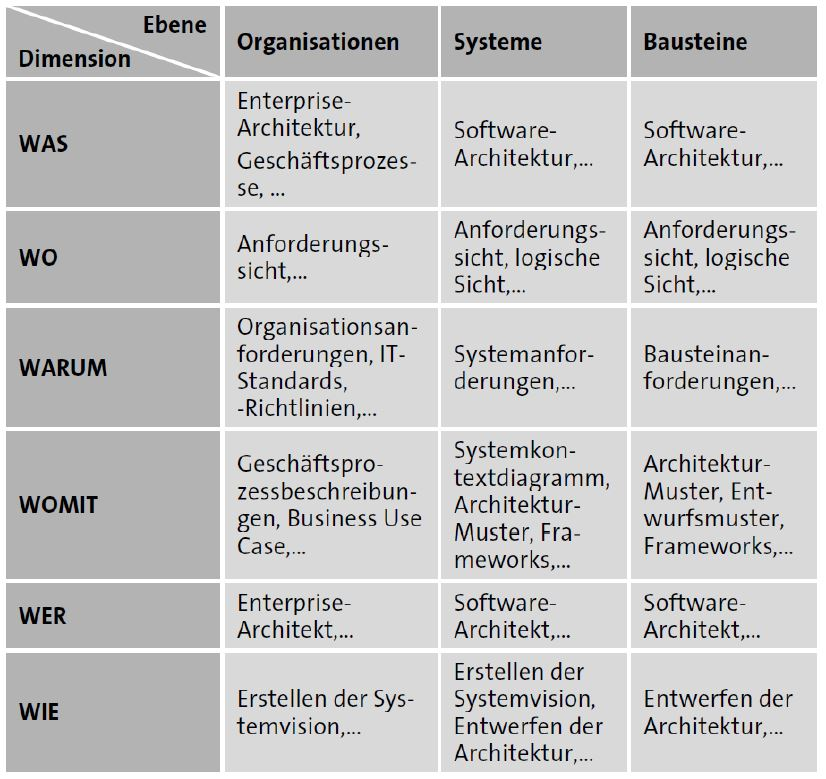
\includegraphics[width=0.5\linewidth]{fig/architekur-ebenen-und-dimensionen}
\caption{Architekur Ebene und Dimensionen}
\label{fig:architekur-ebenen-und-dimensionen}
\end{figure}

Zimmerann unterscheidet nach folgenden Ebenen:
\begin{itemize}
	\item Exekutive Ebene: Architekturstil
	\item Konzeptuelle Ebene: Architekturmuster
	\item Technologie Ebene: Java EE oder .NET?
	\item Hersteller Ebene: IBM oder Oracle
\end{itemize}

\subsection{Dokumentation der Architektur}
Der Architekt dokumentiert seine Ergebnisse oft in ein Dokument mit folgenden Bezeichnungen: Architektur-Gesamtdokument, Architektur-Referenz, Architecture-State-of-the-Art.

Diese enthalten die sogenannten \emph{work products}:
\begin{itemize}
	\item Aufgabenstellung, Anforderungen und Ziele, Stakeholder
	\item Randbedingungen und Kontextsicht
	\item Weitere Sichten, Begriffsglossare
	\item Entwurfsentscheidungen und verwendete Muster
	\item Szenarien zur Architekturbewertung
	\item Risiken, change requests, Projektaspekte
\end{itemize}

Firmen definieren meistens selbst, was sie in einem Architektur-Dokument sehen wollen. Es gibt aber auch diverse Standards: DoDAF, TOGAF, UMF, ARC42, ISO 10746, IEEE 1471/ ISO 42010.

Folgendes gilt es zu beachten, wenn eine gute Dokumentation entstehen soll:
\begin{itemize}
	\item Klarheit schaffen und für einheitliches Verständnis unter Stakeholdern sorgen (Begriffe definieren u. konsistent verwenden)
	\item Dokumentation strukturieren und Struktur kommunizieren
	\item Das Warum dokumentieren: Entscheidungen, Alternativen, Ergebnis mit Begründung.
	\item Redundanz vermeiden
	\item Konsistenz von Diagrammen und Sichten sichern
\end{itemize}

Folgende Fragen sollte eine Dokumentation beantworten:
\begin{itemize}
	\item Wie fügt sich das System in seine Umgebung ein, insbesondere in seine technische Infrastruktur?
	\item Wie ist das System als Menge von Implementierungs-einheiten strukturiert und welche Beziehungen gibt es zwischen diesen?
	\item Wie verhalten sich die Bausteine zur Laufzeit und wie arbeiten sie zusammen?
\end{itemize}

\begin{figure}[h!]
\centering
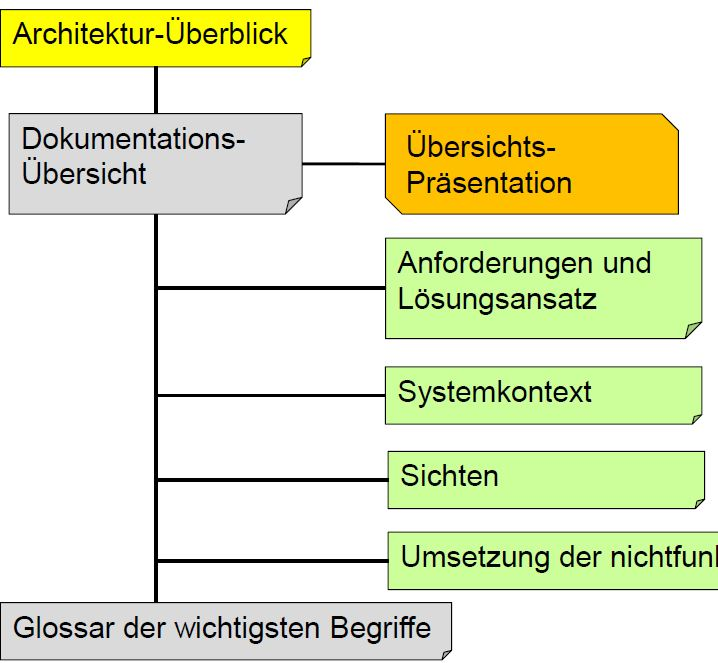
\includegraphics[width=0.5\linewidth]{fig/gute-architektur-dokumentation}
\caption{Gute Architektur Dokumentation}
\label{fig:gute-architektur-dokumentation}
\end{figure}

Eine \textbf{Architekturentscheidung} muss folgende vier Punkte beinhalten: Problem (issue), Alternativen (alternatives), getroffener Entscheid (outcome) und Begründung (rationale). 



\section{Bewertung von Architekturen (ATAM)}

Bei der Bewertung einer Architektur sollte man immer beachten, dass es nicht die gute oder schlechte Architektur gibt. Eine Architektur kann aber besser oder schlechter zu einem Verwendungszweck passen. Softwarearchitektur kann nur qualitativ bewertet werden. Es sind zwar quantitative Messungen möglich (Änderungshäufigkeit der Anforderungen, Testabdeckung, Bugs während Implementierung, Codemetriken usw.), dieser sind aber meist nicht sehr sinnvoll. Vielmehr interessieren uns die Antwort-Metriken (Response Measures) der Szenarien.

Immer wenn eine Schlüssel-Entscheidung getroffen wird oder ein Meilenstein erreicht wird, sollten die gewählten Entscheidungen und mögliche Alternativen analysiert werden (Wie wichtig ist Entscheidung? Wie viele Alternativen gibt es?). Die Kosten der Analyse dürfen natürlich die Kosten einer Fehlerentscheidung nicht übersteigen. Eine Methode um diese Bewertung durchzuführen ist die Architecture Tradeoff Analysis Method (ATAM). Bei ATAM gibt es folgende drei Gruppen von Beteiligten:
\begin{description}
	\item[Evaluatoren:] ausserhalb des Projektes, ATAM Experten
	\item[Projektentscheider:] Architekt, Projekt Leiter, Product Owner
	\item[Architektur Stakeholder:] Haben Interesse an funktionierender Architektur und formulieren deshalb die Qualitätsattribute (Entwickler, Tester, Benutzer).
\end{description}
ATAM ist eigentlich eine Risikoanalyse, welche einen Zusammenhang zwischen den Architekturentscheidungen und dem zu erwarteten Systemverhalten findet. Abbildung \ref{fig:atam} zeigt einen Überblick über die wesentlichen Elemente von ATAM.
\begin{figure}
\centering
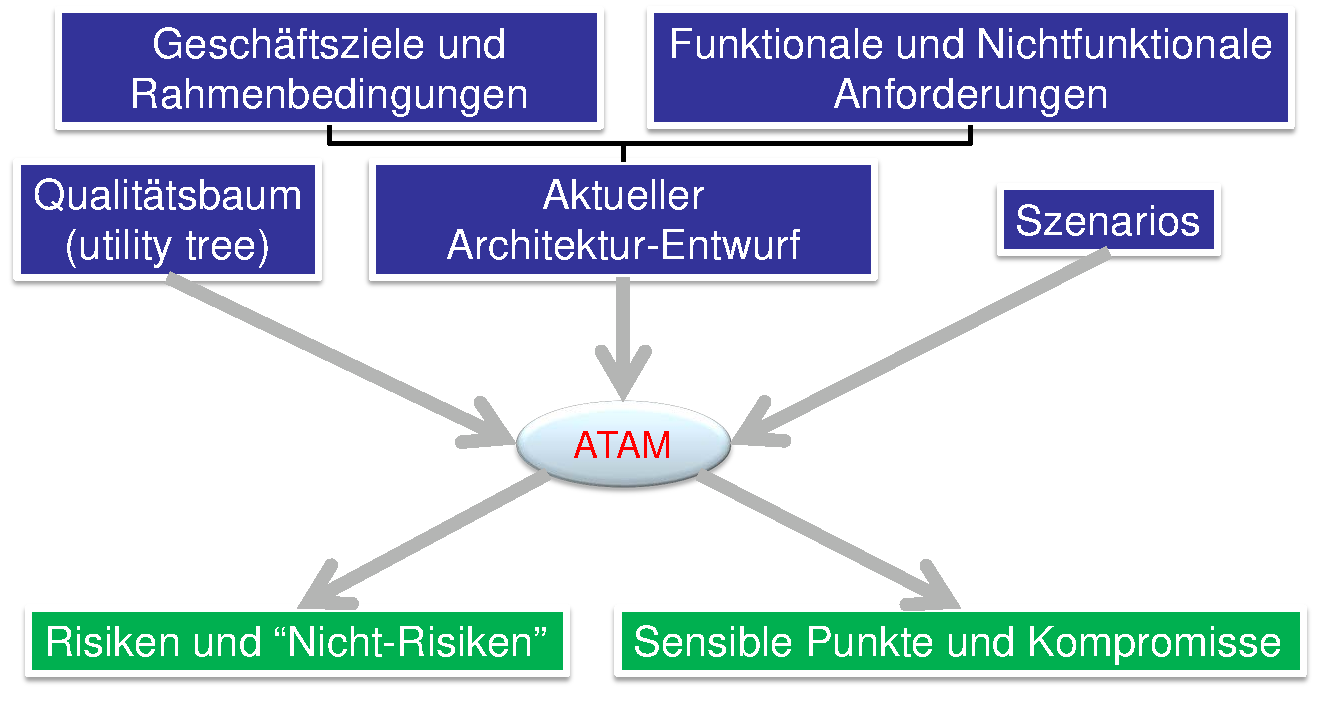
\includegraphics[width=0.6\linewidth]{fig/atam}
\caption{ATAM Übersicht}
\label{fig:atam}
\end{figure}
ATAN läuft nach folgendem Schema ab:
\begin{enumerate}
	\item Stakeholder zusammenbringen
	\item ATAM erklären
	\item Business Driver/Kontext für Systementwicklung zusammenfassen
	\item Architektur vorstellen - Stile sind wichtig
	\item Qualitätsbaum aufbauen
	\begin{enumerate}
		\item Attribute hierarchisieren und Bedeutung quantifizieren
		\item Szenarien definieren und priorisieren
	\end{enumerate} 
	\item Szenarien und Architektur gegenüberstellen
	\item Risiken, sensible Punkte, Kompromisse identifizieren
	\item Massnahmen definieren
\end{enumerate}
Falls die Analyse nicht die gewünschten Ergebnisse liefert oder sich die Anforderungen an das System geändert haben, muss man den Ablauf gegebenenfalls wiederholen. Führt man eine ATAM Analyse korrekt durch ergeben sich folgende Vorteile daraus:
\begin{itemize}
	\item Klärung von nichtfunktionalen Anforderungen und Qualitätsattributen
	\item Verbesserte Dokumentation von Architektur und Architekturentscheidungen
	\item Intensivierte Diskussion zwischen Stakeholdern
	\item Frühe Erkennung von Risiken, wenn früh durchgeführt (RISIKO: ATAM ist zeitaufwendig!)
\end{itemize}
Eine ATAM Analyse liefert folgende Ergebnisse:
\begin{itemize}
	\item Eine präzise und verständliche Darstellung der Architektur
	\item Formulierung der Geschäftsziele
	\item Priorisierte Anforderungen der Qualitätsattribute in Form von Szenarien
	\item Risiken (Eine Architekturentscheidung, die negative Auswirkungen auf ein Szenario hat, ist ein Risiko)
	\item Risikothemen: Welche systematischen Schwächen in der Architektur (oder auch im Team oder im Prozess) führen zu den Risiken?
	\item Beziehung der Architekturentscheidungen zu den Qualitätsattributen
	\item Sensible Punkte und Kompromisse (Architekturentscheidungen mit Auswirkungen auf ein oder mehrere Qualitätsattribute)
\end{itemize}
Zentral sind dabei die nachfolgend beschriebenen Konzepte:

\subsubsection{Qualitätsbaum (Utility Tree)}

Ein Qualitätsbaum stellt die Qualitäten mit den Szenarien in Verbindung. Die Szenarien werden dabei gewichtet (z.B. nach Wahrscheinlichkeit/Auswirkung). Abbildung \ref{fig:utility-tree} zeigt ein Beispiel für einen Qualitätsbaum.

\begin{figure}
\centering
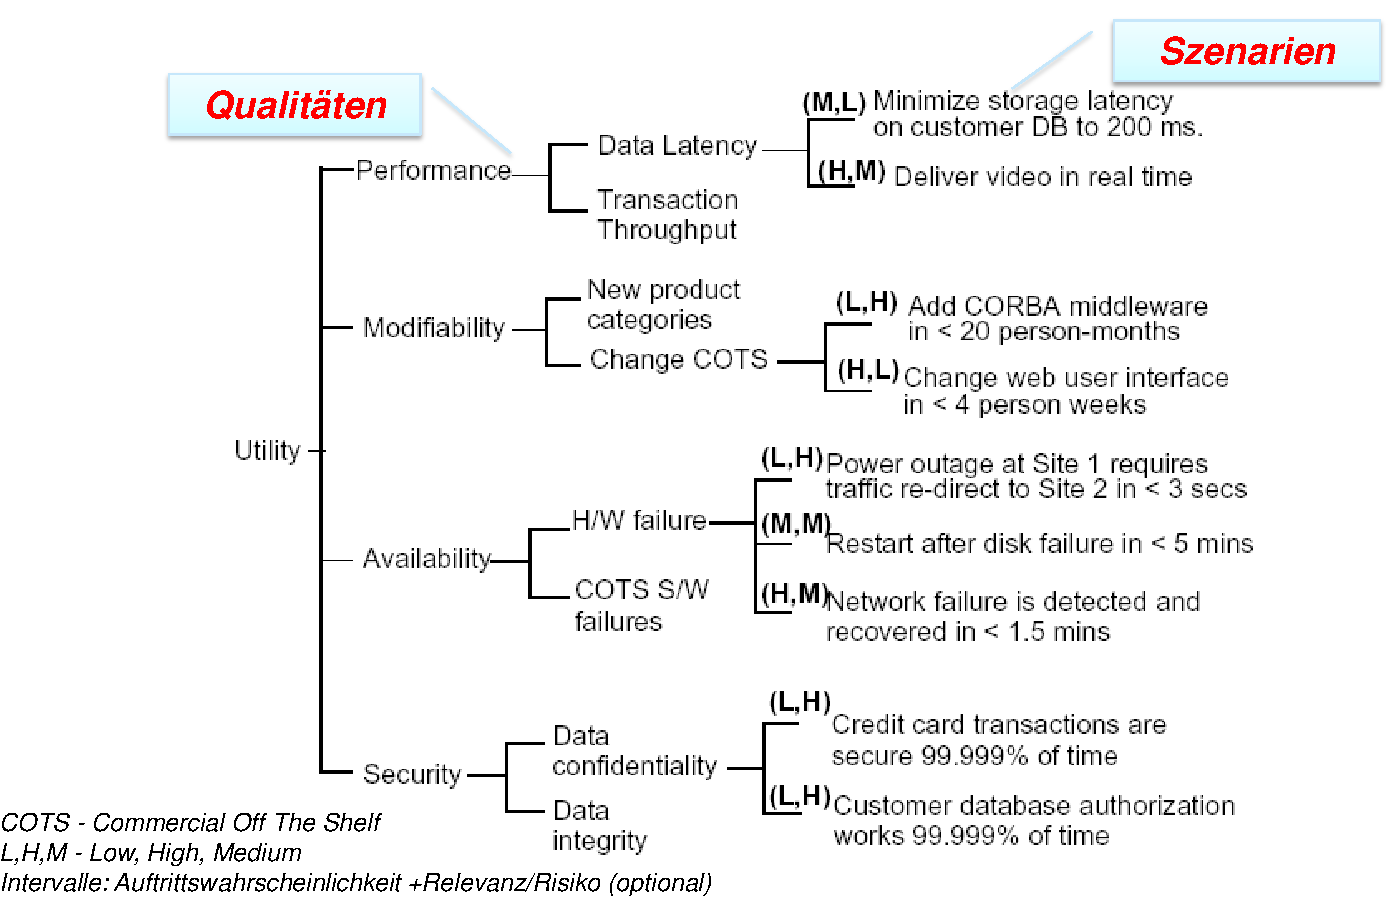
\includegraphics[width=0.7\linewidth]{fig/utility-tree}
\caption{Qualitätsbaum}
\label{fig:utility-tree}
\end{figure}

\subsubsection{Risiken und Nicht-Risiken (Risks/Non-Risks)}

Eine Architekturentscheidung kann entweder ein Risiko für ein Qualitätsattribut sein oder ein Nicht-Risiko wenn die Entscheidung das Qualitätsattribut unterstützt. Nachfolgend je ein Beispiel für ein Risiko und für ein Nicht-Risiko:
\begin{quote}
	Der Backup der Datenbank stellt ein Risiko für die Performanz des Systems dar, wenn eine hohe Systemleistung mit hohen Kosten verbunden ist.
\end{quote}

\begin{quote}
	Der Backup ist kein Risiko bei geringen Kosten für die Systemleistung.
\end{quote}
Ändern sich die Anforderungen an ein System, müssen die Entscheidungen nochmals überprüft werden, weil aus einem Nicht-Risiko ein Risiko werden könnte und umgekehrt.

\subsubsection{Sensible Punkte (Sensitivity Points)}

Sensible Punkte sind Architekturentscheidungen, die bei einer geringfügigen Änderung grosse Auswirkungen auf ein Qualitätsattribut haben. Nachfolgend ein Beispiel für einen sensiblen Punkt:

\begin{quote}
	Der tägliche Backup der Datenbank ist wichtig für die Zuverlässigkeit des Systems.
\end{quote}

\subsubsection{Kompromisse (Tradeoffs)}

Kompromisse sind Architekturentscheidungen, die Auswirkungen auf mehrere Qualitätsattribute haben. Nachfolgend ein Beispiel für einen Kompromiss:

\begin{quote}
	Der Backup der Datenbank sichert die Zuverlässigkeit, aber beeinträchtigt die Performanz des Systems.
\end{quote}

\section{Beruf des IT Architekten}

Der IT-Architekt muss den Prozess des Architekturentwurfs kennen:

\begin{itemize}
	\item Denken in Systemen (Strukturen, Grenzen, Beziehungen)
	\item Anwendung von Prinzipien, Taktiken, Stilen, Mustern
	\item Bewertung des Entwurfs
\end{itemize}

Man soll inkrementell und strukturiert Vorgehen:

\begin{itemize}
	\item Analyse der Anforderungen und Auflösung von Konflikten
	\item Anwendung von Prinzipien, Taktiken \& Mustern
	\item Erzeugen von Modellen \& Prototypen
	\item Bereitstellen von Sichten für Beteiligte
	\item Dokumentation von Entscheidungen
\end{itemize}

Die Lösung ist immer als Kompriss verschiedene Qualitätsattribute zu betrachten. Der Architekt muss also kompromissbereit sein, alle anderen kommen nie ans Ziel. Ein guter Architekt hat folgendes Grundwissen:

\begin{itemize}
	\item Architekturprinzipien
	\item Architekturstile, -taktiken und -muster
	\item Architekturentscheidungen
	\item Architektursichten und Bewertungen
\end{itemize}

\begin{figure}[h!]
\centering
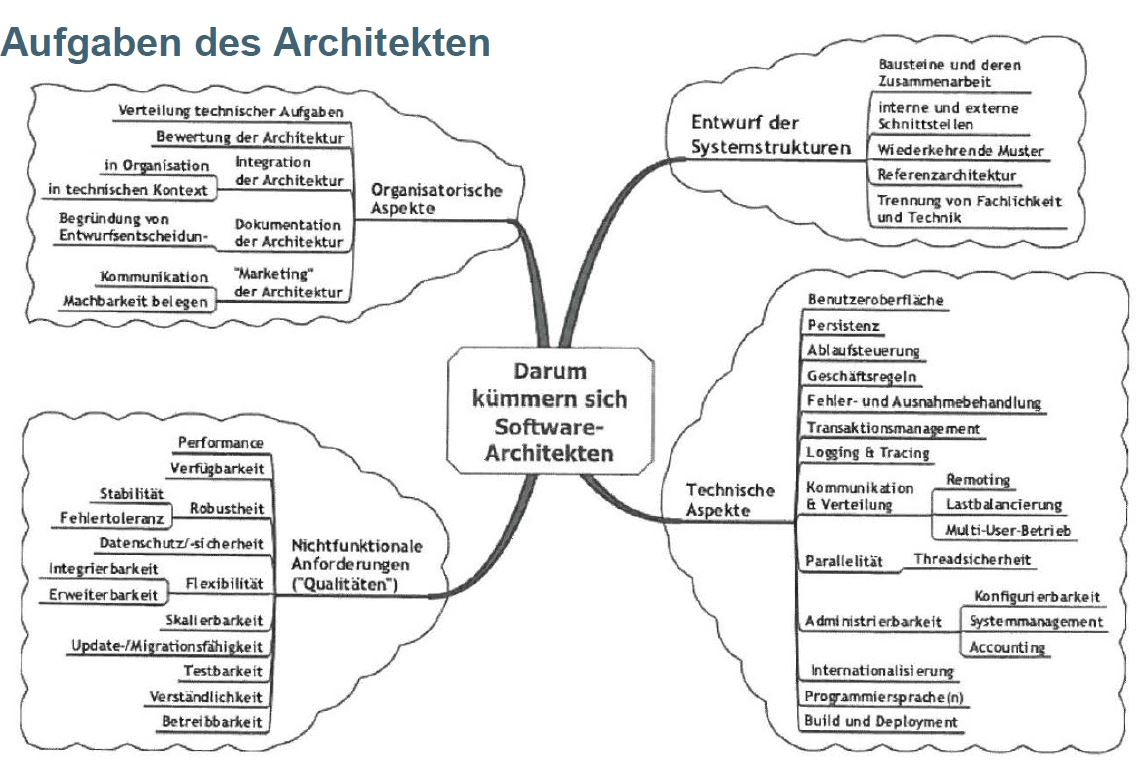
\includegraphics[width=0.7\linewidth]{fig/aufgaben-des-architekten}
\caption{Aufgaben des Architekten}
\label{fig:aufgaben-des-architekten}
\end{figure}

Anforderungen an den Architekten:

\begin{itemize}
	\item Architekturwissen und -erfahrung
	\item Technische Breite und Technologieverständnis
	\item Diszipliniertes, methodenbasiertes Arbeiten
	\item Erfahrung mit dem gesamten Software-Lebenszyklus
	\item Führungsqualitäten und Kommunikationsfähigkeiten
\end{itemize}

Die Häufigsten Fehler:
\begin{itemize}
	\item Glauben der Anforderungen
	\item Technologie-Abhängigkeiten
	\item Fokussieren auf die Stärke und die Schwächen vernachlässigen
	\item Designer designen ewig
	\item Du denkst, dass Du alles alleine machen kannst.
	\item Abgrenzung fehlt
	\item Nicht mit den Stakeholdern reden
	\item Funktionen den Qualitäten bevorzugen
\end{itemize}

Ein guter Architekt lernt von den Erfahrung anderer. Es gibt offizielle Zertifierungsstellen wie die von Open Group.


\section{Fallstudie Fillialbestellsystem aus Modul Applikationsentwicklung}